\documentclass[[12pt,oneside,openany,a4paper, %... Layout
english, %... Global lang drivers{}
masters-t, goldenblock]{usthesis} 
\usepackage{float} %for images
\usepackage{graphicx}
% \usepackage[colorinlistoftodos,prependcaption,textsize=small,disable]{todonotes}
\usepackage[colorinlistoftodos,prependcaption,textsize=small]{todonotes}
\usepackage{pgfgantt}
\usepackage{float} %so that it can use the 'f' float option
\usepackage{pdflscape} %allow you to make landscape pages
\usepackage{amsmath}
\newcommand*\mean[1]{\bar{#1}} % to create an overbar for symbols
% \usepackage{cite}
\usepackage{soul}
\usepackage{amssymb}
\usepackage{bm}
\usepackage{standalone}
\usepackage{preview}
\usepackage{mathtools}
\usepackage{pdfpages}
% \usepackage[sort&compress]{natbib} %able to cite 2 reference at once
\usepackage{cite}
% \usepackage{gensymb} %for degree symbol
% \usepackage{hyperref} %to hyperlink the equations

\newganttlinktype{drur}{
\ganttsetstartanchor{on bottom=0.75}
\ganttsetendanchor{on left}
\draw [/pgfgantt/link]
% first segment (down)
(\xLeft, \yUpper) --
% second segment (right)
(\xLeft, \yUpper -
\ganttvalueof{link bulge} * \ganttvalueof{y unit chart}) --
% link label
node [pos=.5, /pgfgantt/link label anchor] {\ganttlinklabel}
% third segment (up)
($(\xLeft,
\yUpper -
\ganttvalueof{link bulge} * \ganttvalueof{y unit chart})!%
\ganttvalueof{link mid}!%
(\xRight,
\yUpper -
\ganttvalueof{link bulge} * \ganttvalueof{y unit chart})$) --
% last segment (right again)
($(\xLeft, \yLower)!%
\ganttvalueof{link mid}!%
(\xRight, \yLower)$) --
(\xRight, \yLower);
}

\newganttlinktype{rdldr*}{%
  \draw [/pgfgantt/link]
    (\xLeft, \yUpper) --
    (\xLeft + \ganttvalueof{link bulge 1} * \ganttvalueof{x unit},
      \yUpper) --
    ($(\xLeft + \ganttvalueof{link bulge 1} * \ganttvalueof{x unit},
      \yUpper)!%
      \ganttvalueof{link mid}!%
      (\xLeft + \ganttvalueof{link bulge 1} * \ganttvalueof{x unit},
      \yLower)$) --
    ($(\xRight - \ganttvalueof{link bulge 2} * \ganttvalueof{x unit},
      \yUpper)!%
      \ganttvalueof{link mid}!%
      (\xRight - \ganttvalueof{link bulge 2} * \ganttvalueof{x unit},
      \yLower)$) --
    (\xRight - \ganttvalueof{link bulge 2} * \ganttvalueof{x unit},
      \yLower) --
    (\xRight, \yLower);%
}
\ganttset{
  link bulge 1/.link=/pgfgantt/link bulge,
  link bulge 2/.link=/pgfgantt/link bulge}

\begin{document}

\includepdf{Cover.pdf}
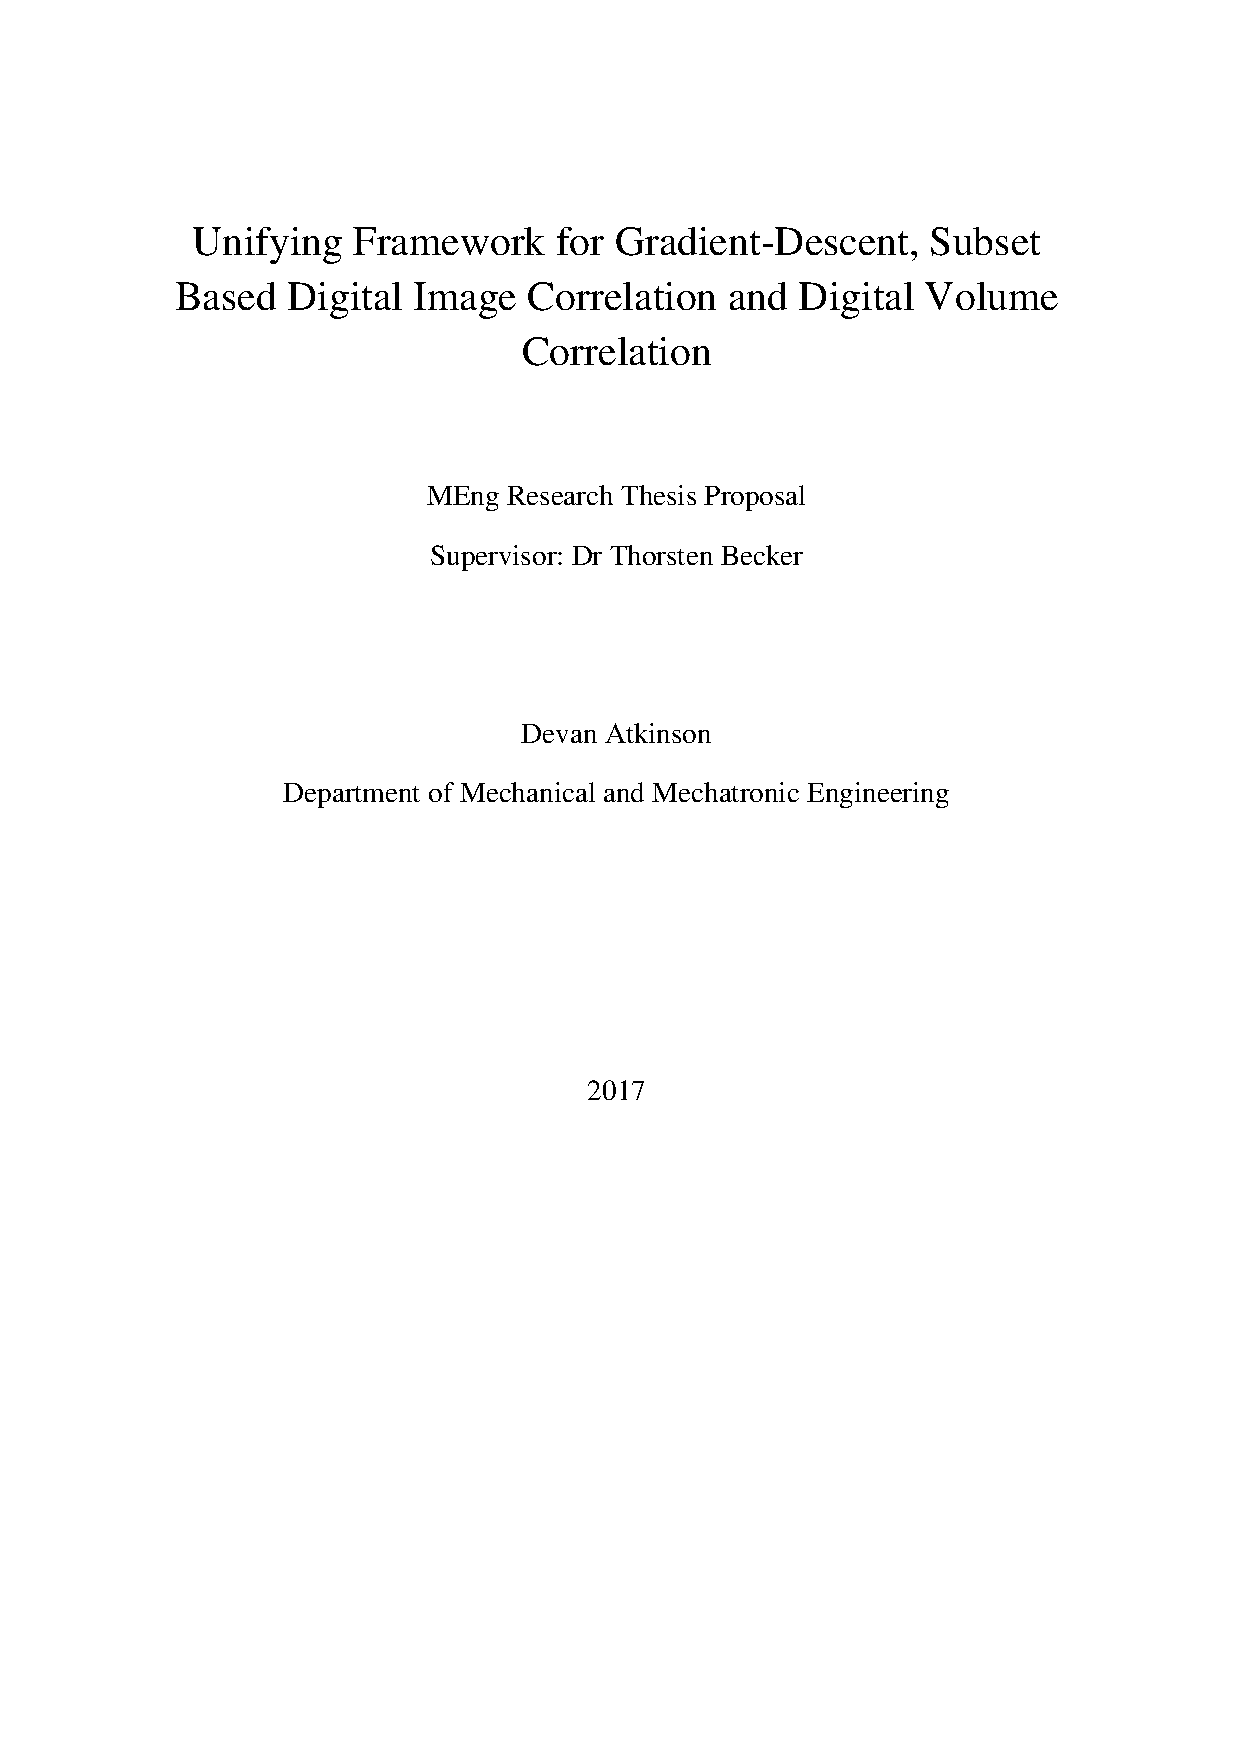
\includepdf{TitlePage.pdf}

\includepdf{plagiarism.pdf}
% \chapter*{Abstract}
% Digital Image Correlation (DIC) and Digital Volume Correlation (DVC) are becoming widely used tools, in the field of material science, to measure the displacements and deformations of specimens. However the high cost of commercial DIC and DVC software and the limited control offered over the correlation process in both commercial and open-source software limits its widespread adoption. This paper proposes a project which aims to create a Matlab based program capable of performing 2D DIC and DVC on a given set of images while allowing the user control over the correlation process. It is hypothesised that the different DIC algorithms use different methods to perform the same tasks in the correlation process. Thus by analysing these algorithms it is possible to combine these different methods into one program which will allow the user to select which methods to use for the various correlation tasks. If successful, this project will produce a freely available program, which offers many of the correlation methods of the different DIC algorithms, so that users will be able to perform in depth DIC and DVC analyses.

% which allows users full control over the correlation process 

% This project primarily consists of researching different DIC algorithms to determine the various methods of performing correlation and incorporating these methods into the program so that the user can choose which to use.



%  This project is motivated by the lack of freely available DIC software which allows the user to control the correlation process. This software is intended to combine most of the 2D DIC algorithms that are beneficial to material science applications into a single code. The successful completion of this project  will allow researchers of material science a comprehensive tool to determine specimen deformation from images taken of the specimen.

\tableofcontents
\listoffigures
\chapter{Introduction}
Digital Image Correlation (DIC) has become a popular tool in the field of material science to measure the deformations and displacements of test specimens as they are loaded. In order to gain a better understanding of the DIC process this project aims to create code in Matlab that is capable of performing the basic elements of DIC. This includes the calibration process, which is used to relate optical flow between images to metric displacements in the real world, and the correlation process which determines the optical flow between images. The purpose of this report is to present the mathematical basis used within the Matlab codes.

\chapter{Theory}
This chapter outlines the theory that is relevant for Digital Image Correlation. First the digital camera is discussed in order to understand how it captures light and stores it as data. Thereafter the optical system, made of a system of lenses and apertures, which focuses the light for the digital camera is reviewed since it has a significant influence on how a three dimensional scene is converted into two dimensional data. Then the camera model that is used to mathematically relate three dimensional coordinates in the real world to two dimensional pixels in the image is presented. Lastly the distortions that are caused by the slight imperfections of lenses are explained. 

\section{Digital cameras}
Cameras at the basic level rely upon using an aperture and a lens to focus light rays that originate from objects onto a plane within the camera called the sensor plane. At the sensor plane exist a Charge-Coupled Device (CCD) that consists of a matrix of light sensors. Each light sensor converts the light incident upon its surface into an electrical charge through the photoelectric effect. The charge is proportional to the light intensity. Then each light sensor's voltage is read by an analogue-to-digital converter which measures the voltage and assigns a digital value to it. These digital values are then stored at the corresponding position in a matrix which forms the digital image.

% Thus for an image of an object to be in focus the light incident upon each light sensor should originate from one point on the object surface. However light is reflected by objects in many directions and so a means of focusing the light is required. This is accomplished through using lenses and an aperture. This is discussed in the next section.

% In order to take an image of an object, such that it is in focus, 

% A point on an object reflects light in all directions and so in order to capture an image of an object, such that it is in focus, the light rays leaving a point on an object must be refocused so that they all intersect at the same point on the sensor plane. 


% If a point on the sensor plane receives light rays from different parts of the object then this will result in a blurry image.
\section{Camera optics}
For an image of an object to be in focus the light incident upon each light sensor should originate from one point on the object's surface. However light is reflected by objects in many directions and so a means of focusing the light is required. This is accomplished through using lenses and an aperture. Throughout this project thin lenses are assumed. A thin lens is one in which its thickness is negligible in comparison with its focal length or radius of curvature \cite{sutton2009image}. Additionally the paraxial approximation is assumed which states that light rays passing through the lens do so with a small angle to the lens's optical axis and pass through the lens close to the optical axis. This leads to the small angle approximation.
\begin{equation}
  \sin(\theta) \approx \tan(\theta) \approx \theta
\end{equation}

Lenses are usually disk shaped pieces of glass with two convex surfaces. The convex surfaces are designed to bend light towards the optical axis with the degree of bending increasing with the distance from the light to optical axis at the lens mid plane. Thus diffuse light emanating from a point M $[x,y,z]^T$ on an object will pass through the lens and the light rays will converge at a point called the ideal image point M' $[x',y',z']^T$. Thereafter the light rays diverge again to points M'' $[x'', y'', z'']^T$ as shown in figure \ref{fig:optics}. If the sensor plane is coincident with the ideal image points of the light rays the image that forms on the sensor is inverted due to the way the lens bends the light. As a result an inverted coordinate system is used for the sensor plane.

\begin{figure}[h]
    \centering
    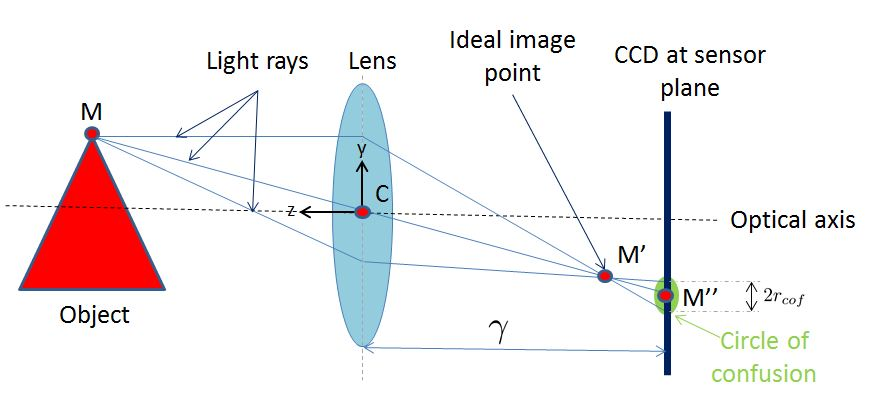
\includegraphics[scale=0.6]{Optics}
    \caption{Illustration of how light rays are manipulated by the lens}
    \label{fig:optics}
\end{figure}

% Due to the way the lens bends the light rays the image formed if the sensor plane is coincident with the resulting in an inverted image M'' (x'',y'',z'') if the sensor plane is behind the ideal image point. Since this is the most common camera configuration an inverted coordinate system is used for the sensor plane.

The thin lens equation can be stated as
\begin{equation}
\frac{1}{|CM|} + \frac{1}{CM'} = \frac{1}{\mean{f}}
\end{equation}
where $\mean{f}$ is the focal length; an inherent property of the lens. Additionally through similarity of triangles we have
\begin{align}
\frac{y}{CM} = \frac{-y'}{CM'}\\
\frac{x}{CM} = \frac{-x'}{CM'}\\
\frac{z}{CM} = \frac{-z'}{CM'}.
\end{align}
Combining these a series of equations for the ideal image point can be obtained.
\begin{align}
\label{eq:optics y'2y}
\begin{split}
x'&=\frac{-\mean{f} x}{z - \mean{f}} \\
y'&=\frac{-\mean{f} y}{z - \mean{f}} \\
z'&=\frac{-\mean{f} z}{z - \mean{f}}
\end{split}
\end{align}

\subsection{Circle of confusion}
It is impossible to align the sensor plane perfectly with the ideal image points and so the divergence of the light rays after the ideal image point causes the light rays to illuminate a circular area on the sensor plane. This blurred region is known as the circle of confusion. If this circular area is larger than the area spanned by an element of the sensor then this will result in blurring in the image as the light spills over multiple sensors. This blur could be eliminated by having the sensor plane the same distance from the lens as the the ideal image point but different points on the object will have different ideal image points.

The light rays that make up the outer perimeter of the circle of confusion are the rays that pass through the lens on the outer edges. Using these rays it is possible to determine the radius of the circle of confusion. Taking $r$ to be the radius of the lens these outer light rays pass through the midplane of the lens at $[r \cos \beta, r \sin \beta, 0]^T$ where $0<\beta<2\pi$. Using trigonometry the y components of these light rays can be related.
\begin{equation}
  \frac{y' - r \sin \beta}{z'}= \frac{y' - y''}{\gamma + z'}
\end{equation}
Th distance between the lens and the sensor plane is given by $\gamma$. The same can be done for the x component. Using this and equation \ref{eq:optics y'2y} an expression for the perimeter of the circle of confusion can be found.
\begin{equation}
\label{eq:cof}
  \begin{bmatrix}
  x'' \\
  y'' \\
  z''
  \end{bmatrix} =
  \begin{bmatrix}
  r \cos \beta + r \cos \beta \left( 1 + \frac{\gamma \left( \mean{f} - z \right)}{\mean{f} z} \right) \\
  r \sin \beta + r \sin \beta \left( 1 + \frac{\gamma \left( \mean{f} - z \right)}{\mean{f} z} \right) \\
  0
  \end{bmatrix} +
  \begin{bmatrix}
  -\frac{\gamma x}{z} \\
  -\frac{\gamma y}{z} \\
  - \gamma
  \end{bmatrix}
\end{equation}
The radius of the circle of confusion can be determine by taking the difference in the y components of $y''$ for $\beta=90 ^{\circ} $ and $\beta=270 ^{\circ}$.

\begin{align}
  2 r_{cof} &= \left[r \sin 90 ^{\circ} \left( 2 + \frac{\gamma \left( \mean{f} - z \right)}{\mean{f} z} \right) \right] - \left[r \sin 270 ^{\circ} \left( 2 + \frac{\gamma \left( \mean{f} - z \right)}{\mean{f} z} \right) \right] \\
  r_{cof}&=r \left( 1 + \frac{\gamma \left( \mean{f} - z \right)}{\mean{f}z} \right)
\end{align}

Another way that the blur can be improved is by using an aperture. An aperture is at a basic level an opaque diaphragm with a hole in it which serves to reduce the amount of light that is incident upon the sensor. Thus by blocking off the light that passed through the outer edges of the lens the aperture reduces the size of the circle of confusion by effectively reducing the radius of the lens. The aperture can be place in front or behind the lens. 

\subsection{Depth of field}
Depth of field is defined as the distance ahead and behind the object that is in focus. For a particular camera system the ideal image point of an object will fall upon the sensor plane if the object is at an ideal focal length from the lens. If the object is any closer or further from the lens it will cause a circle of confusion on the sensor plane as opposed to a point. If the circle of confusion is small enough it will not spill significant light over multiple sensors which will result in a clear image.% be interpreted as a point by the light sensor in which case it is clear in the image.

However if the circle of confusion is large enough it will cause blurring in the image. The largest circle of confusion which still results in a sharp image is referred to as the acceptable circle of confusion \cite{sutton2009image}. Thus the depth of field can be considered as the distance along the z-axis ahead or behind the ideal focus length which results in an acceptable circle of confusion.

The largest degree of freedom for a specific camera system occurs when the object is at the hyperfocal length, $H$, from the camera. The hyperfocal length is defined as the closest an object can be to the camera such that the depth of field extends to infinity behind the object. In this situation the depth of field starts at a distance of $\frac{H}{2}$. The hyperfocal length can be approximated as
\begin{equation}
  H \simeq \frac{\mean{f}^2}{2 N r_{cof}}
  \label{eq:hyperfocal}
\end{equation}
Here $N$ is given by $\frac{\mean{f}}{D_p}$ where $D_p$ is the diameter of the entrance pupil for the camera system. Letting $s$ be the distance from the camera to the object such that the camera is ideally focused at a distance $s$. The distance from the camera to the near limit of the depth of field, $D_N$, and the distance from the camera to the far limit of the depth of field, $D_F$, can be approximated.
\begin{align}
  D_N \simeq \frac{Hs}{H+s} \\
  D_F \simeq \frac{Hs}{H-s}
\end{align}
These approximations assume that the object distance is large compared to the lens focal length. The depth of field can then be determined.
\begin{equation}
  DOF = D_F - D_N = \frac{2 H s^2}{H^2 - s^2}
  \label{eq:DOF}
\end{equation}
Combining equation \ref{eq:hyperfocal} and \ref{eq:DOF} 
\begin{equation}
  DOF = \frac{4 N r_{cof} \mean{f}^2 s^2}{\mean{f}^4 - 4 N^2 r_{cof}^2 s^2}.
\end{equation}
Thus it is clear that the depth of field can be controlled by altering the focal length of the lens, by altering $N$ by changing the aperture or changing the distance between the camera and the object.

\subsection{Field of view}
\todo{viewing frustum}
The field of view is the extent of the world that the camera is capable of capturing in an image. It is quantified as the largest angle that a light ray, that is incident upon the sensor, makes with the optical axis. This angle is referred to as the angle-of-view.

Using the pinhole camera model with a distance of $L$ between the sensor and the lens and taking the lens height to be $d$ a relation for the angle-of-view, $\alpha$, can be derived using trigonometry.
\begin{align}
  \tan \left( \frac{\alpha}{2} \right) &= \frac{d}{2 L} \\
  \alpha &= 2 \arctan \left( \frac{d}{2L} \right)
\end{align}

However for the best picture quality the distance between the sensor and the lens should be equal to the focal length $f$.
\begin{equation}
  \alpha = 2 \arctan \left( \frac{d}{2f} \right)
\end{equation}

\subsection{Transformation to image plane}
The relation between an object point and the projection of the object point onto the sensor can be derived from equation \ref{eq:cof} by eliminating the circle of confusion component. Additionally when the camera system is set up properly $z'$ will be equal to $\gamma$ so that the sensor plane is approximately coincident with the ideal image points. 
\begin{equation}
\label{eq:w2i}
  \begin{bmatrix}
  x'' \\
  y'' \\
  z''
  \end{bmatrix} = 
  \begin{bmatrix}
  -\frac{\gamma}{z} & 0 & 0 \\
  0 & -\frac{\gamma}{z} & 0 \\
  0 & 0 & -\gamma
  \end{bmatrix}
  \begin{bmatrix}
  x \\
  y \\
  1
  \end{bmatrix}
\end{equation}
This equation presents two issues. Firstly the dependence of the sensor positions on $z$. Secondly all the terms in the equation have metric units whereas the image coordinate system has dimensions measured in pixels. These issues are fixed by using a homogeneous from of equation \ref{eq:w2i}.
\begin{equation}
\label{eq:w2ih}
  \alpha \begin{bmatrix}
  -x'' \\
  -y'' \\
  1
  \end{bmatrix} =
  \begin{bmatrix}
  \gamma & 0 & 0 & 0 \\
  0 & \gamma & 0 & 0 \\
  0 & 0 & 1 & 0
  \end{bmatrix}
  \begin{bmatrix}
  x \\
  y \\
  z \\
  1
  \end{bmatrix}
\end{equation}
Here $\alpha$ is a scale factor which allows for the conversion from metric units for the world coordinate system to pixels used in the sensor coordinate system. This equation is referred to as perspective projection \cite{sutton2009image}.

\subsection{Front image plane model}
A new imaging model that is often preferred for computer vision applications can be obtained by translating the sensor plane a distance of $2\gamma$ along the optical axis. In this case the sensor plane is in front of the lens. Treating the sensor coordinates $M''$ of an object as the intersection of the light ray with the sensor plane; equation \ref{eq:w2ih} remains valid for this configuration.

This imaging model is advantageous in that the sensor plane coordinates are no longer inverted. This means that the scene being imaged is also not inverted.

% \begin{itemize}
%   \item intro
%   \item circle of confusion
%   \item M to M''
%   \item aperture
%   \item DOF
%   \item angle of view
%   \item pinhole inversion
% \end{itemize}

% The surfaces are convex such that diffuse light emanating from a point on an object that passes through the lens will converge and intersect at a point called the ideal imaging point. After the ideal imaging point the light rays begin to diverge again. Once this divergence occurs the image becomes inverted. The lens is placed in front of the sensor plane in an attempt to focus the light from each part of the object onto a single light sensor.

% Lenses are usually disk shaped pieces of glass with two convex surfaces. The surfaces are convex such that diffuse light emanating from a point on an object that passes through the lens will converge and intersect at a point called the ideal imaging point. After the ideal imaging point the light rays begin to diverge again. Once this divergence occurs the image becomes inverted. The lens is placed in front of the sensor plane in an attempt to focus the light from each part of the object onto a single light sensor.

% This is illustrated in figure \todo{figure}.

%  which refract light that passes through them to bring the light closer to the usually shaped such that they have convex surfaces that are shaped in such a way that light passing through the lens is refracted towards the optical axis such that  
\section{Coordinate systems}
\label{sec:coord sys}
Images are only capable of storing two dimensional information whereas we live in a three dimensional world. Thus cameras convert three dimensional information from the world coordinate system into two dimensional information in the sensor coordinate system when a picture is taken as shown in figure \ref{fig:coordsys}. The mathematical relationship between these two coordinate systems is discussed here.

\begin{figure}[h]
    \centering
    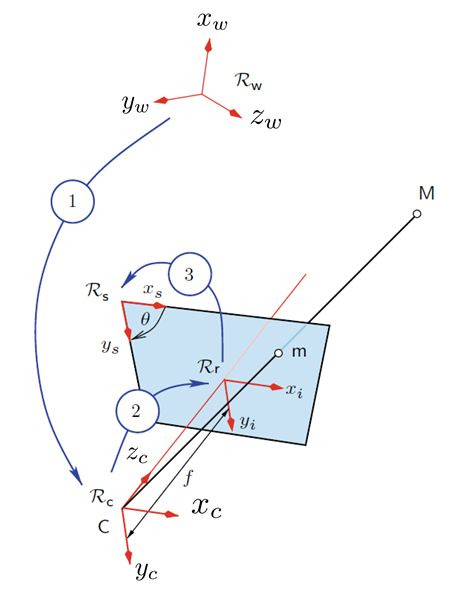
\includegraphics[scale=0.5]{CoordinateSystems}
    \caption{The conversion between coordinate systems that occurs when an image is taken}
    \label{fig:coordsys}
\end{figure}
% Throughout this project thin lenses are assumed. A thin lens is one in which its thickness is negligible in comparison with its focal length or radius of curvature. Additionally the paraxial approximation is assumed which states that light rays passing through the lens do so with a small angle to the lens's optical axis and pass through the lens close to the optical axis. This leads to the small angle approximation.
% \begin{equation}
%   \sin(\theta) \approx \tan(\theta) \approx \theta
% \end{equation}
\todo[inline]{describe how homogeneous coordinates allow n dim vectors to be manipulated in n+1 dim space}
\subsection{Homogeneous coordinates}
It is common knowledge that any object's shape can be fully defined using distances and angles in 3D Euclidean space. However when an image is taken of this object these distances and angles become distorted. For example railway tracks consist of two beams that remain parallel to one another at a set distance apart in Euclidean space but in an image of the railway track (projective space) these beams appear to get closer and closer to one another as seen in figure \ref{fig:traintrack}. Therefore the parallelism between the beams in Euclidean space is distorted in projective space. This occurs as a result of reducing 3D information to a 2D image. \todo{add image}

\begin{figure}[h]
    \centering
    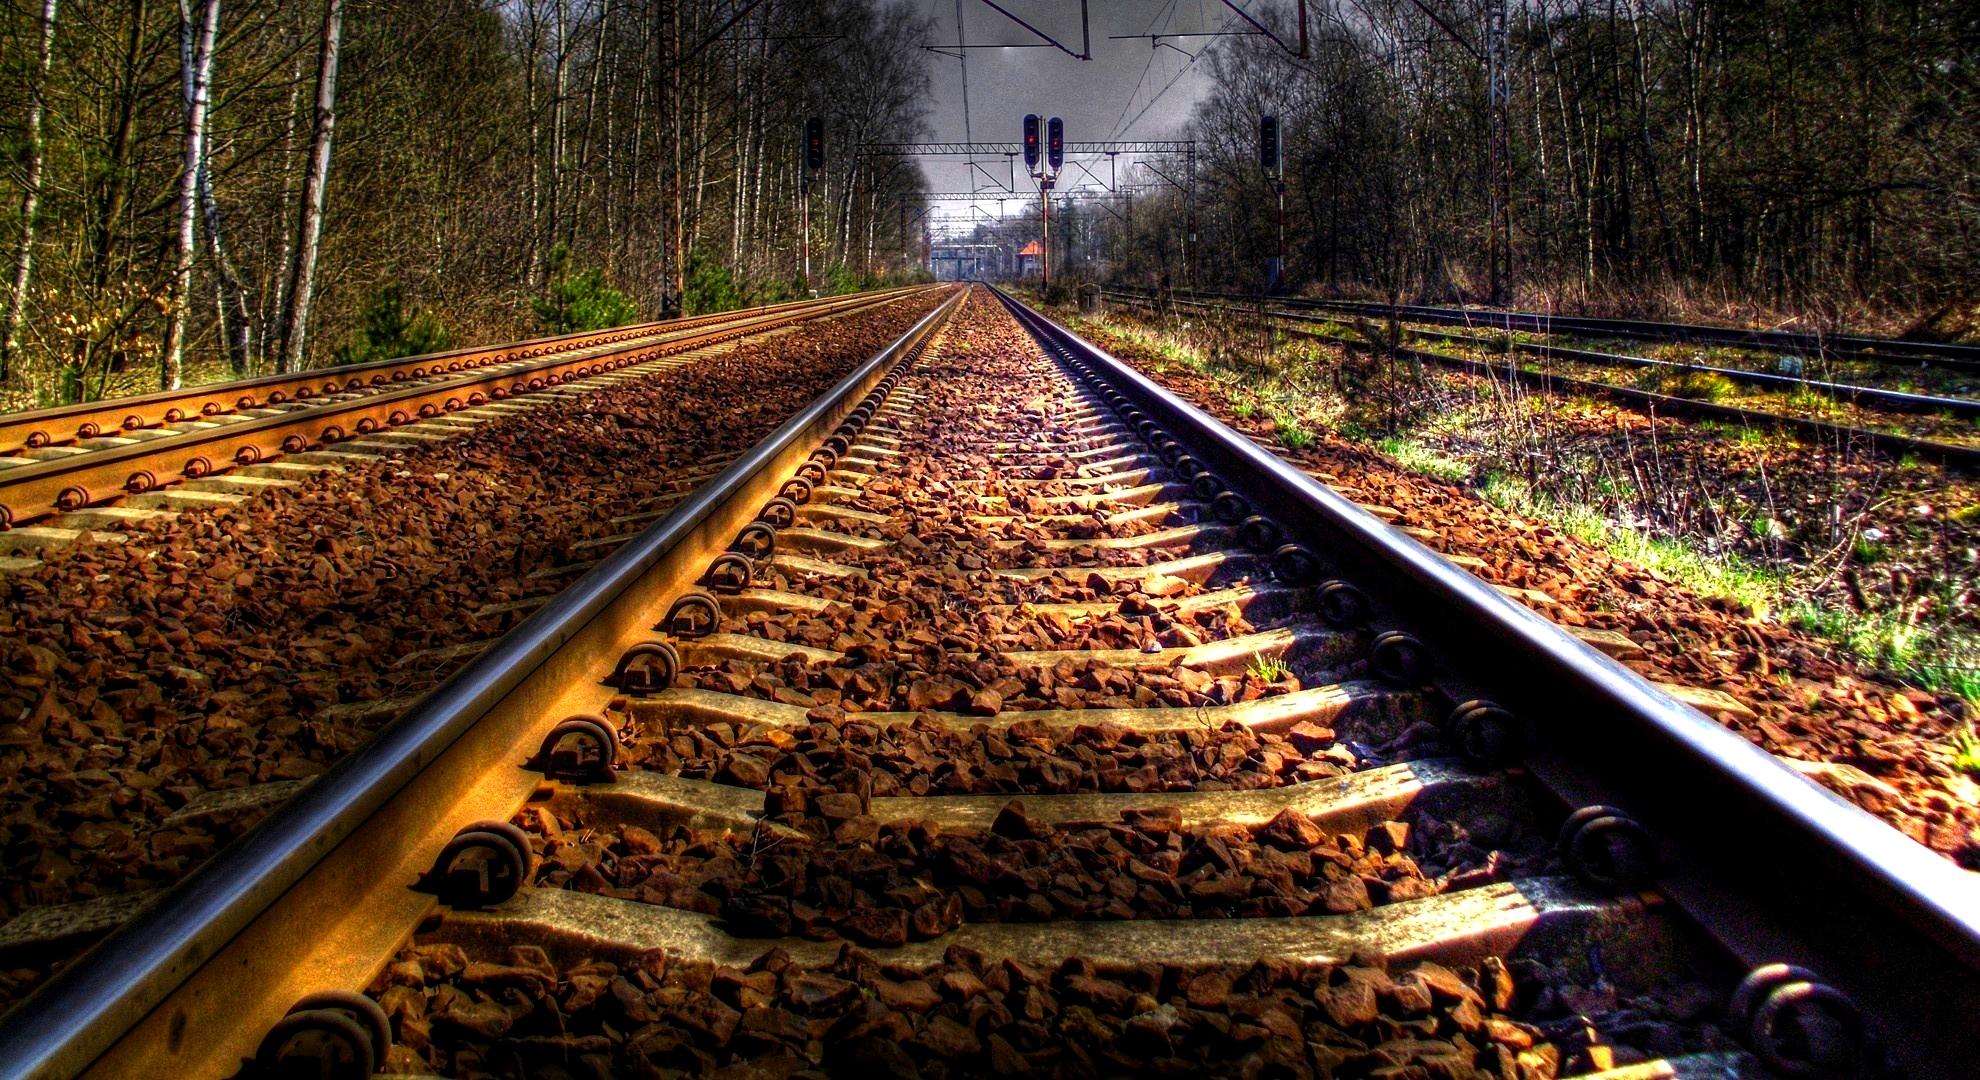
\includegraphics[scale=0.1]{TrainTrack}
    \caption{How projective space distorts parallelism present in Euclidean space}
    \label{fig:traintrack}
\end{figure}

Homogeneous coordinates make it possible to take a 3D coordinate in Euclidean space into a 4D coordinate in projective space. This is necessary since a transformation matrix for 3D coordinates that applies both rotation and translation has 4 columns and so can only be applied to a 4D coordinate. Conversion to homogeneous coordinates involves adding an additional coordinate $w$ to the coordinate vector and setting $w=1$. To convert back from homogeneous coordinates requires dividing the $x$, $y$ and $z$ coordinates by $w$ and then eliminating $w$.

\todo{do a 2D example}
% http://www.songho.ca/math/homogeneous/homogeneous.html
% http://www.tomdalling.com/blog/modern-opengl/explaining-homogenous-coordinates-and-projective-geometry/
\subsection{World to camera coordinate system}
Converting from the world coordinate system to the camera coordinate system involves rigid transformations of translation $T$ and rotation $R$. The world coordinate system is simply the coordinate system that would be used to classify the position and orientation of objects in the real world. The world coordinate systems orientation and origin is somewhat arbitrary and it is usually classified according to the object to be imaged. 

The camera coordinate system is as the name suggests fixed according to the cameras position and orientation. The camera coordinate system's z axis is the optical axis of the camera. The conversion between the two coordinate systems can be represented as
\begin{equation}
  \bm{X}_c = 
  \begin{bmatrix}
  x_c \\
  y_c \\
  z_c \\
  1
  \end{bmatrix}
  =
  \begin{bmatrix}
  r_{11} & r_{12} & r_{13} & t_1 \\
  r_{21} & r_{22} & r_{23} & t_2 \\
  r_{31} & r_{32} & r_{33} & t_3 \\
  0 & 0 & 0 & 1
  \end{bmatrix}
  \begin{bmatrix}
  x_w \\
  y_w \\
  z_w \\
  1
  \end{bmatrix} = 
  \begin{bmatrix}
  \bm{R} & \bm{T} \\
  \bm{0} & 1
  \end{bmatrix} \bm{X}_w.
\end{equation}
\todo{change T and R to lowercase}
Scaling of dimensions between the two coordinate systems also needs to be taken into account. The parameters in $\bm{R}$ and $\bm{T}$ are referred to as extrinsic parameters since they are not dependent on the camera system's hardware but rather the camera's position and orientation in the world coordinate system.

\subsection{Camera and imaging plane coordinates}
The 3D object defined in the camera coordinate system is converted to its projection on imaging plane. This conversion is from a 3D coordinate system to a 2D coordinate system as given below using homogeneous coordinates.
\begin{equation}
\label{eq:c2i}
  \bm{X}_p = \alpha
  \begin{bmatrix}
  x_p \\
  y_p \\
  1
  \end{bmatrix} 
  = 
  \begin{bmatrix}
  \gamma & 0 & 0 & 0 \\
  0 & \gamma & 0 & 0 \\
  0 & 0 & 1 & 0
  \end{bmatrix}
  \begin{bmatrix}
  x_c \\
  y_c \\
  z_c \\
  1
  \end{bmatrix}
\end{equation}
The variable $\alpha$ is an arbitrary scale factor.

\subsection{Image plane and sensor coordinates}
At this point the locations of where the light rays originating from the object will intersect the imaging plane are known. Now it is necessary to mathematically represent how the sensor would interpret these light rays incident upon the sensor into the form of pixels. In order to do this a relation between the position of a point within a coordinate system and the pixel within an image is necessary. Additionally the sensor array is not guaranteed to the orthogonal and so a skewed coordinate system must be taken into account.

The transformation from the image plane coordinate system to a temporary skewed coordinate system with an angle of $\phi$ between the two axes can be represented by
\begin{equation}
\label{eq:plane2skew}
  \begin{bmatrix}
  x_{temp} \\
  y_{temp} 
  \end{bmatrix} =
  \begin{bmatrix}
  1 & -\cot \phi \\
  0 & \frac{1}{\sin \phi}
  \end{bmatrix}
  \begin{bmatrix}
  x_p\\
  y_p
  \end{bmatrix}.
\end{equation}
It is assumed that the two principle directions in the sensor coordinate system have different scale factors, $S_x$ and $S_y$,which have units of pixels per unit length. Applying these to the coordinates calculated in equation \ref{eq:plane2skew} and accounting for the translations $\hat c_x$ and $\hat c_y$ to convert to the origin of the sensor coordinate system results in the sensor coordinates below.
\begin{equation}
  \begin{bmatrix}
  x_s \\
  y_s
  \end{bmatrix} = 
  \begin{bmatrix}
  S_x & 0\\
  0 & S_y
  \end{bmatrix}
  \begin{bmatrix}
  x_{temp}\\
  y_{temp}
  \end{bmatrix} -
  \begin{bmatrix}
  S_x \hat c_x - S_x \hat c_y \cot \phi \\
  \frac{S_y \hat c_y}{\sin \phi}
  \end{bmatrix}=
  \begin{bmatrix}
  S_x & -S_x \cot \phi \\
  0 & \frac{S_y}{\sin \phi}
  \end{bmatrix}
  \begin{bmatrix}
  x_p \\
  y_p
  \end{bmatrix} -
  \begin{bmatrix}
  S_x \hat c_x - S_x \hat c_y \cot \phi \\
  \frac{S_y \hat c_y}{\sin \phi}
  \end{bmatrix}
\end{equation}

This can be rewritten in homogeneous form so that it is consistent with equation \ref{eq:c2i}.
\begin{equation}
  \bm{X}_s = 
  \begin{bmatrix}
  x_s \\
  y_s \\
  1
  \end{bmatrix} =
  \begin{bmatrix}
  S_x & -S_x \cot \phi & -S_x \left( \hat c_x - \hat c_y \cot \phi \right) \\
  0 & \frac{S_y}{\sin \phi} & -\frac{S_y \hat c_y}{\sin \phi} \\
  0 & 0 & 1
  \end{bmatrix}
  \begin{bmatrix}
  x_p \\
  y_p \\
  1
  \end{bmatrix} =
  \bm{A} \bm{X}_i
\end{equation}
\todo{talk about these parameters being intrinsic and combine them better}

\subsection{World to sensor coordinates}
The conversions between coordinate systems described in the previous sections can be combined into one conversion from the world coordinate system to the sensor coordinate system.
\begin{equation}
  \bm{X}_s = \alpha
  \begin{bmatrix}
  x_s \\
  y_s \\
  1
  \end{bmatrix} =
  \begin{bmatrix}
  S_x & -S_x \cot \phi & -S_x \left( \hat c_x - \hat c_y \cot \phi \right) \\
  0 & \frac{S_y}{\sin \phi} & -\frac{S_y \hat c_y}{\sin \phi} \\
  0 & 0 & 1
  \end{bmatrix}
  \begin{bmatrix}
  \gamma & 0 & 0 & 0 \\
  0 & \gamma & 0 & 0 \\
  0 & 0 & 1 & 0
  \end{bmatrix}
  \begin{bmatrix}
  r_{11} & r_{12} & r_{13} & t_1 \\
  r_{21} & r_{22} & r_{23} & t_2 \\
  r_{31} & r_{32} & r_{33} & t_3 \\
  0 & 0 & 0 & 1
  \end{bmatrix}
  \begin{bmatrix}
  x_w \\
  y_w \\
  z_w \\
  1
  \end{bmatrix}
\end{equation}

This can be simplified by combining the first two matrices.
\begin{align}
  \bm{X}_s = \alpha
  \begin{bmatrix}
  x_s \\
  y_s \\
  1
  \end{bmatrix} =
  \begin{bmatrix}
  \gamma S_x & -\gamma S_x \cot \phi & -S_x \left( \hat c_x - \hat c_y \cot \phi \right) & 0\\
  0 & \frac{\gamma S_y}{\sin \phi} & -\frac{S_y \hat c_y}{\sin \phi} & 0\\
  0 & 0 & 1 & 0
  \end{bmatrix}
  \begin{bmatrix}
  r_{11} & r_{12} & r_{13} & t_1 \\
  r_{21} & r_{22} & r_{23} & t_2 \\
  r_{31} & r_{32} & r_{33} & t_3 \\
  0 & 0 & 0 & 1
  \end{bmatrix}
  \begin{bmatrix}
  x_w \\
  y_w \\
  z_w \\
  1
  \end{bmatrix}
  \label{eq:world 2 sensor cumbersome}
\end{align}

Replacing the elements of the first matrix in equation \ref{eq:world 2 sensor cumbersome} with single variables for the purposes of simplicity the equation can be rewritten as

\begin{align}
  \alpha
  \begin{bmatrix}
  x_s \\
  y_s \\
  1
  \end{bmatrix} &=
  \begin{bmatrix}
  f_x & f_s & c_x & 0\\
  0 & f_y & c_y & 0\\
  0 & 0 & 1 & 0
  \end{bmatrix}
  \begin{bmatrix}
  r_{11} & r_{12} & r_{13} & t_1 \\
  r_{21} & r_{22} & r_{23} & t_2 \\
  r_{31} & r_{32} & r_{33} & t_3 \\
  0 & 0 & 0 & 1
  \end{bmatrix}
  \begin{bmatrix}
  x_w \\
  y_w \\
  z_w \\
  1
  \end{bmatrix} \\
  &= \bm{K} \bm{V} \bm{X}_w.
  \label{eq:world 2 sensor}
\end{align}
Here the parameters relating the world coordinate system to the sensor coordinate system are separated into two matrices. The first matrix $\bm{K}$ contains the intrinsic parameters which are fixed for a specific camera. The second matrix $\bm{V}$ contains the extrinsic parameters. The extrinsic parameters change when the camera's position and orientation relative to the world coordinate system changes.
\todo{explain this better}

\section{Distortion}
Distortion refers to a collection of phenomena that cause the actual image to differ from that of the idealised image expected from the pinhole camera model. This happens because lenses cannot be manufactured and assembled perfectly and so some misalignment and defects exist in the imaging system. Therefore in order to calculate accurate displacement information the distortions must be accounted for and corrected prior to the correlation process.

Distortion can be separated into many types as done below. The overall distortion of the image can then be mathematically represented as the linear combination of the mathematical expressions for the individual types. A brief explanation of each distortion type and the equation that accounts for the distortion it creates is given below.
% https://www.lensrentals.com/blog/2010/10/the-seven-deadly-aberrations/

\subsection{Spherical distortion}
Spherical distortion is when light rays originating from a point on an object intersect at different points on the sensor plane. This is as a result of the lens not having the perfect curvature required for all the light rays to intersect at the same point on the sensor plane. It is assumed to be axis symmetric relative to the axis passing through the centre of the sensor and to be a function of the radial distance.
\begin{equation}
  \bm{D} = \kappa_1 \rho ^4 \bm{e}_r
\end{equation}
Here $\bm{e}_r$ is the radial unit vector and $\rho$ is the distance from the origin of the sensor coordinate system to the point under consideration.

\subsection{Coma distortion}
Coma distortion affects light rays that travel towards the lens at an angle to the optical axis. Light rays that go through the centre portion of lens refocus to a point on the sensor plane, whereas light rays that pass through the outer portion of the lens don't refocus fully and intersect the sensor plane further (positive coma) or closer (negative coma) to the optical axis. This results in light from a point on an object creating a comet-like shape on the sensor plane. It is corrected with the following equation.
\begin{equation}
  \bm{D} = \kappa_2 \rho^3 \cos \left( \mean{\theta} - \mean{\theta_c} \right) \bm{e}_r
\end{equation}
Here $\mean{\theta_c}$ is the orientation of the projected lens tilt angle in the sensor plane.

\subsection{Astigmatism}
Astigmatism is caused by a lens having curvature that varies when measured along perpendicular planes. For instance the vertical plane of the lens has a different curvature to the horizontal plane of the lens. The different curvatures have different focal lengths and so light passing through the vertical portion of the lens will focus at a different distance from the lens than light that passes through the horizontal portion of the lens. This results in line like blurs on the sensor plane for the curvature that is not in focus. The degree to which the astigmatism affects the image increases further away from the centre of the image.
\begin{equation}
  \bm{D} = \kappa_3 \rho^2 \cos \left( \mean{\theta} - \mean{\theta}_A \right) \bm{e}_r
\end{equation}
Where $\mean{\theta}_A$ is the orientation of the projected astigmatic plane within the sensor plane.

\subsection{Curvature of field}
Curvature of field is a distortion that results due to the curved nature of the optical elements such as the lens. As light rays pass through the lens with a small angle to the optical axis they refocus at the sensor plane. However light rays that pass through the lens at a larger angle to the optical axis refocus at a point that is closer to the lens. This results in the light rays refocusing on a curved plane much like a shallow dome. Since the sensor is planar (flat) this causes the centre of the image to be in focus while the edges of the image are not in focus.

Curvature of field is assumed to be symmetric with respect to the optical axis and to be a quadratic function of the radial position \cite{sutton2009image}.
\begin{equation}
  \bm{D}=\kappa_4 \rho^2 \bm{e}_r
\end{equation}
Here $\kappa_4$ is the amplitude of the curvature of distortion in the sensor plane measured in $\text{pixels}^{-1}$.
% https://photographylife.com/what-is-field-curvature

\subsection{Linear}
This non-symmetric distortion component is assumed to be a linear function of radial position and is dependent on the angular position \cite{sutton2009image}.
\begin{equation}
  \bm{D} = \kappa_5 \rho \cos \left( \mean{\theta} - \mean{\theta_L} \right) \bm{e}_r
\end{equation}
Here $\mean{\theta_L}$ is the angular orientation of the linear distortion axis.

\subsection{Radial}
Radial distortion is caused by the lens having different magnification levels based on the angle of the light rays to the optical axis. As a result the image can experience a decrease in magnification with increasing distance from the optical axis (barrel distortion) or the image can experience increasing magnification with increasing distance from the optical axis (pincushion distortion). This distortion is symmetric with respect to the optical axis.
\begin{equation}
  \bm{D} = \kappa_6 \rho ^3 \bm{e}_r + \kappa_7 \rho^5 \bm{e}_r + \kappa_8 \rho^7 \bm{e}_r
\end{equation}
% http://www.shariblog.com/2013/08/difference-between-barrel-pincushion-distortion/
% https://photographylife.com/what-is-distortion
\subsection{De-centering}
De-centering distortion is caused by the lens not being in perfect alignment with the rest of the camera system. Usually this type of distortion is less severe than radial or spherical distortions.
\begin{equation}
  \bm{D} = \kappa_9 \rho^2 \left[ 3 \sin \left( \mean{\theta} - \mean{\theta_d} \right) \bm{e}_r + \cos \left( \mean{\theta} - \mean{\theta_d} \right) \bm{e}_t \right]
\end{equation}
Here $\bm{e}_t$ is the tangential unit vector and $\mean{\theta_d}$ is the orientation of the axis for maximum tangential distortion.

% http://www.pcigeomatics.com/geomatica-help/concepts/orthoengine_c/Chapter_47.html

















\chapter{Calibration}
Calibration is a necessary process that must be completed in order to extract metric information from images. The calibration process solves for parameters that define the optical characteristics of the camera, parameters that define the orientation and position of the camera coordinate system to the world coordinate system and parameters that define the distortions that must be corrected for in the images. By determining all of these parameters the calibration process will have solved the camera model that predicts how an object in three dimensional space is related to the pixel, which containing the light reflected by the object, in the image captured of the object.

The parameters that define the optical characteristics and the distortions are referred to as intrinsic parameters since they are fixed for a specific camera. The parameters that describe the orientation and position of the camera within the world coordinate system are extrinsic parameters because they change if the camera is moved. \todo{explain intrinsic and extrinsic better}

Multiple methods of calibration exist however calibration using a calibration plate is used in this project since it is one of the most popular methods and manufacturing a calibration plate is relatively simple and inexpensive.

\section{Inverse problem}
Calibration is essentially a method of finding the parameters that allow 3D coordinates in the world coordinate system to be accurately related to 2D coordinates in the image coordinate system. Thus the inputs, 3D world coordinates, and outputs, 2D image coordinates, needed to be used to solve for the parameters which describe the relationship between the two which constitutes an inverse problem.

Inverse problems are typlically hard to solve and calibration is no exception. In order to solve for the calibration parameters more reliably the camera model that relates world points to sensor points is broken down to the simple pinhole camera model initially in order to solve for as few parameters as possible in the beginning. These parameters are solved for using a closed form solution which gives good estimates to the parameters. Thereafter once these parameters have been estimated the camera model is made more complex by introducing radial distortion in order to account for imperfections in the lens system of the camera. These radial parameters are first estimated and now with each parameter having a corresponding estimate all the parameters are optimized simultaneously in an iterative manner.

This inverse problem is sensitive to errors in the 3D world coordinates (inputs) and 2D image coordinates (outputs) used. Thus these need to be known to a high degree of accuracy in order to solve for the intrinsic and extrinsic camera parameters reliably. This is achieved by using a calibration plate.

\section{Calibration plate}
A calibration plate is an object with a flat surface containing a high-contrast, regular pattern. The pattern is such that it contains definitive, point-like features which can be located to a high degree of accuracy within images taken of it. For example a checker board pattern allows for accurate calculation of the points at the corners of the squares. Thus the coordinates of these point-like features on the calibration plate will be known (inputs) and the coordinates of these point-like features in the image can be determined to a high degree of accuracy (outputs). These definitive, point-like features are hereafter referred to as calibration targets.

Since images inherently contain some level of noise it is best to have an overdetermined system of equations. This is accomplished by taking multiple images of the calibration plate and changing the relative position and orientation between the calibration plate and the camera for each image. This effectively reduces the effects of noise; making the system more robust.

\section{Homography}
\label{sec: homography}
Homography is a transformation that can be applied to points on a plane to bring it into alignment with another plane. It is used to bring the calibration targets on the calibration plate in the world coordinate system into alignment with their location in the image in the sensor coordinate system. The transformation from world coordinates to sensor coordinates in equation \ref{eq:world 2 sensor} is a type of homography.

Treating the calibration plate such that it lies in the x-y plane of the world coordinate system; the homography, $\bm{H}$, for calibration is given by the following equation.
\begin{equation}
  \begin{bmatrix}
  x_s \\
  y_s \\
  1
  \end{bmatrix} = 
  \alpha
  \begin{bmatrix}
  f_x & f_s & c_x & 0\\
  0 & f_y & c_y & 0\\
  0 & 0 & 1 & 0
  \end{bmatrix}
  \begin{bmatrix}
  r_{11} & r_{12} & r_{13} & t_1 \\
  r_{21} & r_{22} & r_{23} & t_2 \\
  r_{31} & r_{32} & r_{33} & t_3 \\
  0 & 0 & 0 & 1
  \end{bmatrix}
  \begin{bmatrix}
  x_w \\
  y_w \\
  0 \\
  1
  \end{bmatrix} \\
\end{equation}
Since the calibration targets are set to lie on the x-y plane within the world coordinate system this eqaution can be reduced to 
\begin{align}
  \begin{bmatrix}
  x_s \\
  y_s \\
  1
  \end{bmatrix} &=
  \alpha
  \begin{bmatrix}
  f_x & f_s & c_x \\
  0 & f_y & c_y \\
  0 & 0 & 1 
  \end{bmatrix}
  \begin{bmatrix}
  r_{11} & r_{12} & t_1 \\
  r_{21} & r_{22} & t_2 \\
  r_{31} & r_{32} & t_3 
  \end{bmatrix}
  \begin{bmatrix}
  x_w \\
  y_w \\
  1
  \end{bmatrix} \\
  &= \alpha \bm{K} 
  \begin{bmatrix}
  \bm{r}_1 & \bm{r}_2 & \bm{t}
  \end{bmatrix}
  \begin{bmatrix}
  x_w \\
  y_w \\
  1
  \end{bmatrix} \\
  &= \alpha
  \begin{bmatrix}
  h_{11} & h_{12} & h_{13} \\
  h_{21} & h_{22} & h_{23} \\
  h_{31} & h_{32} & h_{33}
  \end{bmatrix} 
  \begin{bmatrix}
  x_w \\
  y_w \\
  1
  \end{bmatrix}
  =\alpha \bm{H} 
  \begin{bmatrix}
  x_w \\
  y_w \\
  1
  \end{bmatrix} \label{eq: homography 1}
\end{align}
Here $\bm{r}_1$ and $\bm{r}_2$ are the first and second columns of the rotation matrix. It is clear that the homography matrix contains both intrinsic and extrinsic parameters and thus it is different for each image taken of the calibration plate. Additionally note that the homography matrix is defined up to a scale factor $\alpha$.

%http://www.learnopencv.com/homography-examples-using-opencv-python-c/

\section{Estimating homography with direct linear transformation}
The homographies that relate the world coordinates of the calibration plate targets to the targets in the image can be estimated using direct linear transformation (DLT) \cite{zhangtut}. Equation \ref{eq: homography 1} can be written out as
\begin{align}
  x_s &= \alpha \left( h_{11} x_w + h_{12} y_w + h_{13} \right) \label{eq: homo line 1} \\
  y_s &= \alpha \left( h_{21} x_w + h_{22} y_w + h_{23} \right) \label{eq: homo line 2} \\
  1 &= \alpha \left( h_{31} x_w + h_{32} y_w + h_{33} \right) \label{eq: homo line 3}.
\end{align}
The scale factor, $\alpha$, can be eliminated by dividing equations \ref{eq: homo line 1} and \ref{eq: homo line 2} by \ref{eq: homo line 3} to get
\begin{align}
  x_s \left( h_{31} x_w + h_{32} y_w + h_{33} \right) &= \left( h_{11} x_w + h_{12} y_w + h_{13} \right) \\
  y_s \left( h_{31} x_w + h_{32} y_w + h_{33} \right) &= \left( h_{21} x_w + h_{22} y_w + h_{23} \right)
\end{align}
These equations then reduce to
\begin{align}
  - h_y x_w x_s - h_{32} y_w x_s + h_{11} x_w + h_{12} y_w +h_{13} &= h_{33} x_s \label{eq: solve homo 1}\\
  - h_{31} x_w y_s - h_{32} y_w y_s + h_{21} x_w + h_{22} y_w + h_{23} &= h_{33} y_s. \label{eq: solve homo 2}
\end{align}
In order to avoid the trivial solution where every element in the homogrpahy matrix is equal to zero; constraints need to be placed on the elements of the homography matrix. In this case the element $h_{33}$ is set equal to 1 however other constraints are also possible such as $h_{31}^2 + h_{32}^2 + h_{33}^2 = 1$. Note that if the true value of $h_{33}$ is close to zero then this assumption will introduce a singluarity \cite{emerging}.

Each calibration target, having points $x_{w_i}$ and $y_{w_i}$, on the calibration plate that is captured within an image of the calibration plate, having points $x_{s_i}$ and $y_{s_i}$, provides two relations of the form of equations \ref{eq: solve homo 1} and \ref{eq: solve homo 2}. These equations are then stacked together into an equation of the form
\begin{align}
  \begin{bmatrix}
  x_{w_1} & y_{w_1} & 1 & 0 & 0 & 0 & -x_{w_1} x_{s_1} & -y_{w_1} x_{s_1} \\
  0 & 0 & 0 & x_{w_1} & y_{w_1} & 1 & -x_{w_1} y_{s_1} & -y_{w_1} y_{s_1} \\
  x_{w_2} & y_{w_2} & 1 & 0 & 0 & 0 & -x_{w_2} x_{s_2} & -y_{w_2} x_{s_2} \\
  0 & 0 & 0 & x_{w_2} & y_{w_2} & 1 & -x_{w_2} y_{s_2} & -y_{w_2} y_{s_2} \\
  \vdots & \vdots & \vdots & \vdots & \vdots & \vdots & \vdots & \vdots 
  \end{bmatrix}
  \begin{bmatrix}
  h_{11} \\
  h_{12} \\
  h_{13} \\
  h_{21} \\
  h_{22} \\
  h_{23} \\
  h_{31} \\
  h_{32}
  \end{bmatrix} =
  \begin{bmatrix}
  x_{s_1} \\
  y_{s_1} \\
  x_{s_2} \\
  y_{s_2} \\
  \vdots
  \end{bmatrix}
  \label{eq:DLT}
\end{align}
This overdetermined system of equations then can be used to solve for the homography matrices of each calibration image using least squares. This is the first step involved in calibration.

% http://www.kwon3d.com/theory/dlt/dlt.html

\subsection{Direct linear transformation normalisation}
In practice the use of the DLT method to find estimates to the homographies was found to be sensitive to noise in the images. It was discovered by R. Hartley \cite{DLTnorm} that the DLT method can be made much more robust to noise by applying translation and scaling to the image and world coordinate points prior to performing DLT. Specifically the sensor and world coordinate points are first translated such that the origin of each coordinate system is located at the centroid of the points defined in that coordinate system. Then the coordinates are scaled such that the average distance of the coordinates from the origin is equal to $\sqrt{2}$. This scaling and translation has the effect of reducing the condition number of the matrix in equation \ref{eq:DLT}.

The translation and scaling of the coordinates is done separately for the sensor and world coordinates as shown with $\bm{X_{w}'}$ and $\bm{X_{s}'}$ representing the transformed and scaled versions of the world and sensor coordinate points respectively.
\begin{align}
  \bm{X_{w}'} &= \bm{T_w} \bm{X_w} \\
  \bm{X_{s}'} &= \bm{T_s} \bm{X_s}
\end{align}

Since different coordinate points are used for DLT the homography computed, $\bm{H'}$, is not the homography of the original coordinate pairs, $\bm{H}$. However the homography calculated can be transformed back in order to obtain the desired homography matrix.
\begin{equation}
  \bm{H} = \bm{T_{s}^{-1}} \bm{H'} \bm{T_{w}}
\end{equation}

\section{Absolute conic}
\label{sec: abs conic}
As mentioned before two objects that are parallel in Euclidean space appear to intersect each other in projective space. The intersection of these two lines in projective space occurs at a point that lies on the plane at infinity. If a point lies upon the plane at infinity its $w$ is equal to zero in homogeneous coordinates.

The absolute conic lies on the plane at infinity and is defined by the set of points, $\tilde{\bm{x}}_{ac} = [x, y, z, w]^T$, that satisfies the following. 
\begin{align}
  w = 0 \\
  \bm{x}_{ac}^T \bm{x}_{ac}=x^2 + y^2 + z^2 = 0 
  \label{eq:conditions of absolute conic}
\end{align}
Here tilde is used to indicate homogeneous coordinates (projective space) whereas $\bm{x}_{ac} = [x, y, z]^T$ would be the point in Euclidean space.

Thus it is this conic of purely imaginary points that lies upon the plane at infinity. The importance of the absolute conic is that it is invariant under any Euclidean transformations. In other words the relative position of the absolute conic to a moving camera is unaffected by extrinsic parameters. Consider a point $\bm{x}_{ac}$ in Euclidean space in the world coordinate system that lies on the absolute conic. It has homogeneous coordinates $\tilde{\bm{x}}_{ac}=[\bm{x}_{ac}^T, 0]^T$ in projective space. Applying a different rotation and translation to this point to obtain $\tilde{\bm{x}}_{ac}'$, which is equivalent to moving the camera in the world coordinate system, a corresponding point is obtained in the camera coordinate system.
\begin{align}
  \tilde{\bm{x}}_{ac}' &=
  \begin{bmatrix}
  \bm{R} & \bm{T} \\
  \bm{0} & 1
  \end{bmatrix}
  \tilde{\bm{x}}_{ac} =
  \begin{bmatrix}
  r_{11} & r_{12} & r_{13} & t_1 \\
  r_{21} & r_{22} & r_{23} & t_2 \\
  r_{31} & r_{32} & r_{33} & t_3 \\
  0 & 0 & 0 & 1
  \end{bmatrix}
  \begin{bmatrix}
  x_{ac} \\
  y_{ac} \\
  z_{ac} \\
  0
  \end{bmatrix} \\
  &= 
  \begin{bmatrix}
  \bm{R} \bm{x}_{ac} \\
  0
  \end{bmatrix}
\end{align}
It is clear that this point still lies on the plane at infinity since its $w$ is equal to zero. More importantly it can be proven that this point $\bm{x}_{ac}'$ is on the same absolute conic.
\begin{equation}
  \bm{x}_{ac}'^T \bm{x}_{ac}' = \left( \bm{R} \bm{x}_{ac} \right) ^T \left( \bm{R} \bm{x}_{ac} \right) = \bm{x}_{ac}^T \bm{R}^T \bm{R} \bm{x}_{ac} = \bm{x}_{ac}^T \bm{x}_{ac} = 0
\end{equation}
Thus the absolute conic is invariant to Euclidean transformations. Now consider again a point, $\bm{x}_{ac}$, lying on the absolute conic. The corresponding point, $\bm{m}_s$, in the sensor plane is given by
\begin{align}
  \tilde{\bm{m}}_s &= \frac{1}{\alpha} \bm{K} 
  \begin{bmatrix}
  \bm{R} & \bm{T} \\
  \bm{0} & 1
  \end{bmatrix}
  \begin{bmatrix}
  \bm{x}_{ac} \\
  0
  \end{bmatrix} = \frac{1}{\alpha} \bm{K}
  \begin{bmatrix}
  \bm{R} \bm{x}_{ac} \\
  0
  \end{bmatrix} \\
  \therefore \bm{m}_s &= \frac{1}{\alpha} \bm{K} \bm{R} \bm{x}_{ac}.
\end{align}
Checking whether this point satisfies equation \ref{eq:conditions of absolute conic} results in
\begin{equation}
  \bm{m}_s^T \bm{K}^{-T} \bm{K}^{-1} \bm{m}_s = \frac{1}{\alpha^2} \bm{x}_{ac}^T \bm{R}^T \bm{R} \bm{x}_{ac} = \frac{1}{\alpha^2} \bm{x}_{ac}^T \bm{x}_{ac} = 0
\end{equation}
Thus the image of the absolute conic is itself an absolute conic. \todo{absolute or imaginary conic?} The image of the absolute conic is defined by $\bm{K}^{-T} \bm{K}^{-1}$ \cite{luong1997self}. Thus since the image of the absolute conic is dependent only on intrinsic camera parameters it can be used to solve for the intrinsic camera parameters.

% http://www.cs.unc.edu/~marc/tutorial/node87.html
\section{Constraints on intrinsic parameters}
\label{sec: intrinsic constraints}
According to Zhang \cite{emerging} there are two constraints placed upon the intrinsic parameters of the camera. These are important later on in the solving for these intrinsic parameters. The plane of the calibration plate in the camera coordinate system is given by \cite{emerging} 
\begin{equation}
  \begin{bmatrix}
  \bm{r}_3 \\
  \bm{r}_3^T \bm{t}
  \end{bmatrix}^T
  \begin{bmatrix}
  x \\
  y \\
  z \\
  w
  \end{bmatrix} = 0.
\end{equation}
Here $w$ is zero for points on the plane at infinity and one for those that are not. This plane intersects the plane at infinity on a line and it happens that $[\bm{r}_1^T, 0]^T$ and $[\bm{r}_2^T, 0]^T$ are points on this line \cite{emerging}. Thus it is known that any point on this line, $x_c^{\infty}$, is a linear combination of these two points.
\begin{equation}
  x_c^{\infty} = a \begin{bmatrix}
  \bm{r}_1 \\
  0
  \end{bmatrix} + b
  \begin{bmatrix}
  \bm{r}_2 \\
  0
  \end{bmatrix} =
  \begin{bmatrix}
  a \bm{r}_1 + b \bm{r}_2 \\
  0
  \end{bmatrix}
\end{equation}
Now assume that this point, $x_c^{\infty}$, lies on the absolute conic. Then this point must satisfy equation \ref{eq:conditions of absolute conic}. This would require that $a^2+b^2=0$ which results in the solution $b=\pm a i$, where $i=\sqrt{-1}$. As a result it can be seen that the two points along this line intersect the absolute conic at
\begin{equation}
  x_c^{\infty} = a 
  \begin{bmatrix}
  \bm{r}_1 \pm i \bm{r_2} \\
  0
  \end{bmatrix}.
\end{equation}
Since these points lie on the absolute conic they are invariant under Euclidean transformations. Their projection, up to a scale factor, in the sensor coordinate system is given by
\begin{equation}
  x_s^{\infty} = \bm{K} \left( \bm{r}_1 \pm \bm{r}_2 \right) = \bm{h}_1 \pm i \bm{h}_2.
\end{equation}
Substituting these points into equation \ref{eq:conditions of absolute conic} results in
\begin{equation}
  \left( \bm{h}_1 \pm i \bm{h}_2 \right)^T \bm{K}^{-T} \bm{K}^{-1} \left( \bm{h}_1 \pm i \bm{h}_2 \right) = 0.
\end{equation}
Requiring both the imaginary and real parts of this equation to equal zero results in two constraints on the intrinsic camera parameters.
\begin{align}
  \label{eq:intrinsic constraints 1}
  \bm{h}_1^T \bm{K}^{-T} \bm{K}^{-1} \bm{h}_2 &= 0 \\
  \label{eq:intrinsic constraints 2}
  \bm{h}_1^T \bm{K}^{-T} \bm{K}^{-1} \bm{h}_1 &= \bm{h}_2^T \bm{K}^{-T} \bm{K}^{-1} \bm{h}_2
\end{align}
Where $\bm{h}_i = [h_{i1} \, h_{i2} \, h_{i3}]^T$ is the i\textsuperscript{th} column of the homography matrix.

\section{Intrinsic parameters and the absolute conic}
\label{sec: parameters and the absolute conic}
An homography, $\bm{H}$, between the calibration plate and the image of the calibration plate can be estimated. This homography can then be used to solve for the image of the absolute conic. Once the image of the absolute conic is known it can be used to solve for the intrinsic camera parameters. The image of the absolute conic can be represented as
\begin{equation}
  \bm{B} = \bm{K}^{-T} \bm{K}^{-1} = 
  \begin{bmatrix}
  b_{11} & b_{12} & b_{13}\\
  b_{12} & b_{22} & b_{23} \\
  b_{13} & b_{23} & b_{33}
  \end{bmatrix}
\end{equation}
Since $\bm{B}$ is symmetric its contents can be represented by a 6D vector $\bm{b}=[b_{11} \, b_{12} \, b_{22} \, b_{13} \, b_{23} \, b_{33}]^T$. Then
\begin{equation}
  \bm{h}_I^T \bm{B} \bm{h}_j = \bm{v}_{ij} \bm{b}
\end{equation}
where 
\begin{equation}
  \bm{v}_{ij} = [ h_{i1} h_{j1}, h_{i1} h_{j2} + h_{i2} h_{j1}, h_{i2} h_{j2}, h_{i3} h_{j1} + h_{i1} h_{j3}, h_{i3} h_{j2} + h_{i2} h_{j3}, h_{i3} h_{j3}]^T.
\end{equation}
Then equations \ref{eq:intrinsic constraints 1} and \ref{eq:intrinsic constraints 2} can be rewritten as 
\begin{equation}
  \begin{bmatrix} 
  \bm{v}_{12}^T \\
  ( \bm{v}_{11} - \bm{v}_{22})^T
  \end{bmatrix} \bm{b} = \bm{0}
\end{equation}
A separate version of this equation exist for each image taken of the calibration plate and these equations can be stacked, in $\bm{V}$, to give
\begin{equation}
  \bm{V}\bm{b}=\bm{0}.
\end{equation}
The solution for $\bm{b}$, up to a scale factor $\lambda$, is known to be the eigenvector of $\bm{V}^T\bm{V}$ associated with the smallest eigenvalue \cite{emerging}. Once b has been determined it can be used to determine the intrinsic parameters of matrix $\bm{K}$. The relation between $\bm{B}$ and $\bm{K}$ is $\bm{B}=\lambda \bm{K}^{-T} \bm{K}^{-1}$. The intrinsic parameters are determined as follows.
\begin{align}
  c_y &= (b_{12} b_{13} - b_{11} b_{23})/(b_{11} b_{22} - b_{12}^2) \\
  \lambda &= b_{33} -(b_{13}^2 + c_y(b_{12} b_{13} - b_{11} b_{23}))/b_{11}\\
  f_x &= \sqrt{\frac{\lambda}{b_{11}}} \\
  f_y &= \sqrt{\frac{\lambda b_{11}}{b_{11} b_{22} - b_{12}^2}} \\
  f_s &= \frac{-b_{12} f_x^2 f_y}{\lambda} \\
  c_x &= \frac{f_s c_y}{f_y} - \frac{b_{13} f_x^2}{\lambda}
\end{align}
Thereafter the extrinsic parameters can be determined.
\begin{align}
  \bm{r}_1 &= \lambda \bm{K}^{-1} \bm{h}_1 \\
  \bm{r}_2 &= \lambda \bm{K}^{-1} \bm{h}_2 \\
  \bm{r}_3 &= \bm{r}_1 \times \bm{r}_2 \\
  \bm{T} &= \lambda \bm{K}^{-1} \bm{h}_3
\end{align}
At this point it is necessary to incorporate distortions and use them to find better approximations for the intrinsic and extrinsic parameters.

\todo{this section is too close to the paper} %a fleixible new technique and reading 1
% by which the optical characteristics of a camera and the relation between its coordinate system and the world coordinate system are determined. It is performed in order to be able to extract \hl{metric} information from images accurately.

% \section{Closed form solution}
% Sections \ref{sec: homography} through to \ref{sec: parameters and the absolute conic} illustrate that estimates to the intrinsic and extrinsic parameters can be obtained by first determining the homographies for each calibration image, then these can be used to determine the image of the abolute conic which in turn can be used to determine the intrinsic and extrinsic camera parameters. This is closed form solution is the first part of the calibration process

% put inverse problem in calibration plate section

% explain homography and absolute conic

% then explain closed form solution and optimization - give closed form and explain optimization


\section{Distortion in Calibration}
Sections \ref{sec: homography} through \ref{sec: parameters and the absolute conic} outline the framework for the closed form solution of the calibration problem when distortion is not considered. It is only once the closed form solution to the extrinsic and intrinsic parameters is optimised that distortion can be accounted for during the calibration process. As already presented, there are many types of distortion that occur when an image is taken. However it is seldom possible to take all of these distortion types into account since the more distortion parameters introduced into the camera model; the more likely the optimization process becomes unstable.

It has been found \todo{add reference for this} that good calibration results can be achieved by taking only radial distortion into account during calibration \cite{tsai1987versatile,wei1994implicit}. This is beneficial since it is possible to solve for initial guesses to the radial distortion parameters which helps the optimisation process to avoid local minima as a result of the distortion parameters used.

The distortion applied to the points on the image plane is of the form
\begin{align}
  \hat{\bm{X_{p_i}}} =
  \begin{bmatrix}
  \hat{x_{p_i}} \\
  \hat{y_{p_i}}
  \end{bmatrix} &= \left(
  1 + k_1 r^2 + k_2 r^4 \right)
  \begin{bmatrix}
  x_{p_i} \\
  y_{p_i}
  \end{bmatrix}
  = D 
  \begin{bmatrix}
  x_{p_i} \\
  y_{p_i}
  \end{bmatrix}\\
  \text{where} \quad \quad r_i &= \sqrt{x_{p_i}^2 + y_{p_i}^2} \quad \text{and} \quad D=\left(
  1 + k_1 r^2 + k_2 r^4 \right).
\end{align}
Here $\hat{\bm{X_{p_i}}} = \begin{bmatrix} \hat{x_{p_i}} & \hat{y_{p_i}} \end{bmatrix} ^T$ represent the distorted image coordinates.

At this point the intrinsic and extrinsic parameters have been determined using the pinhole camera model and the error between the predicted calibration plate targets and the actual location of these in the images is attributed to radial distortion \cite{zhangtut}. This error is represented as the observed distortion vector $\bm{d_{1_i}}$.
\begin{equation}
  \bm{d_{1_i}} = \bm{X_{s_i}}^{a} - \bm{X_{s_i}}^{c}
\end{equation}
Here $\bm{X_{s_i}}^{a}$ is the actual coordinates observed and $\bm{X_{s_i}}^{c}$ is the predicted coordinates that are calculated according to the camera model.

An undistorted point, $\bm{X_{p_i}}$ is distorted to point $\hat{\bm{X_{p_i}}}$ according to
\begin{align}
  \hat{\bm{X_{p_i}}} &= \bm{U_c} + (\bm{X_{p_i}}-\bm{U_c}) \times (1 + k_1 r_i^2 + k_2 r_i^4) \\
  &= \bm{U_c} + \bm{X_{p_i}} - \bm{U_c} + (\bm{X_{p_i}}-\bm{U_c}) \times (k_1 r_i^2 + k_2 r_i^4) \\
  &= \bm{X_{p_i}} + (\bm{X_{p_i}}-\bm{U_c}) \times (k_1 r_i^2 + k_2 r_i^4) \\
  &= \bm{X_{p_i}} + \bm{d_{2_i}}
\end{align}
Here $\bm{U_c} = \begin{bmatrix} u_c & v_c \end{bmatrix}^T$ is the projection centre or principal point (the intersection of the optical axis with the image plane) and $\bm{d_{2_i}}$ is referred to as the model distortion vector.

The distortion parameters can be estimated by minimizing the difference between the model and observer distortion vectors. Thus the least squares solution to the overdetermined system of equations of the form $\bm{d_{2_i}} = \bm{d_{1_i}}$ is what is needed. For each point $\bm{X_{p_i}}$ considered there are two equations of the form
\begin{align}
  (x_{p_i} - u_c) \times (k_1 r_i^2 + k_2 r_i^4) &= (x_{s_i}^{a} - x_{s_i}^{c}) \\
  (y_{p_i} - v_c) \times (k_1 r_i^2 + k_2 r_i^4) &= (y_{s_i}^{a} - y_{s_i}^{c}).
\end{align}
Two equations of this form are created for each target of the calibration plate and these equations are then stacked into a system of equations which is used to solved for the least squares solution to the distortion parameters.
\begin{equation}
  \begin{bmatrix}
    (x_{p_1} - u_c) \times r_1^2 & (x_{p_1} - u_c) \times r_1^4\\
    (y_{p_1} - v_c) \times r_1^2 & (y_{p_1} - v_c) \times r_1^4\\
    (x_{p_2} - u_c) \times r_2^2 & (x_{p_2} - u_c) \times r_2^4\\
    (y_{p_2} - v_c) \times r_2^2 & (y_{p_2} - v_c) \times r_2^4\\
    \vdots & \vdots
  \end{bmatrix}
  \begin{bmatrix}
    k_1 \\
    k_2
  \end{bmatrix} =
  \begin{bmatrix}
    x_{s_1}^{a} - x_{s_1}^{c}\\
    y_{s_1}^{a} - y_{s_1}^{c}\\
    x_{s_2}^{a} - x_{s_2}^{c}\\
    y_{s_2}^{a} - y_{s_2}^{c}\\
    \vdots
  \end{bmatrix}
\end{equation}

\section{Non-linear optimisation}
At this point good approximations have been calculated for all the calibration parameters using closed form solution methods. However, since the correlation process relies upon the calibration process to link optical flow in images to displacement in the 3D world, these calibration parameters need to be refined so that they don't negatively affect the correlation results. This is done by combining the camera model and distortion into one mathematical relation that related 3D coordinates in the physical world to 2D coordinates in the images. It is important to note that the distortion model is inserted into the camera model prior to converting the image plane coordinates to the sensor plane coordinates. Thus the camera model becomes
\begin{equation}
  \bm{X_s}=\bm{K} D \bm{V} \bm{X_w}.
\end{equation}
This camera model and the approximations of the calibration parameters are employed in a non-linear optimization scheme in order to improve all of the calibration parameters simultaneously. Matlab's built in Levenberg-Marquart non-linear least squares optimisation algorithm was used for this. The sum of the absolute of the difference between the calculated and observed calibration plate targets was used as a measure of the error for the algorithm.

% However these estimates need to be improved upon in order to obtain the true calibration parameter values. This is done by using a non-linear optimisation scheme in order to improve all of the parameters simultaneously. Thus the camera model is combined with the distortion model to obtain one mathematical model of the image capturing system. The Levenberg-Marquart non-linear least squares optimisation algorithm was used to iteratively improve the calibration parameters.

\chapter{Correlation}
The Lucas-Kanade algorithm was used in combination with the zero-mean normalised sum of squared differences correlation criteria. This correlation criteria was chosen since it takes into account offset and scaling in the light intensities of the images making the overall algorithm more robust. The Lucas-Kanade algorithm assumes that the deformation of the image is constant over a area of the image referred to as the subset. As such this algorithm tries to find the deformation field that best corrects a subset of the deformed image so that it appears to be the same as the reference image. 

\section{Correspondence problem and speckle patterns}
Although subsets of pixels are usually easier to track than individual pixels, using subsets leads to a new issue. The correspondence problem is to do with the inability to track displacements as a result of the grayscale patterns within the image. To understand this consider the aperture problem which is a special case of the correspondence problem.

The aperture problem involves the ambiguity in attempting to track the motion of a one-dimensional spatial structure (such as a line) when viewed through an aperture (such as when considering a subset of pixels) that cuts off the view of the ends of the one-dimensional spatial structure \cite{apertureProblem}. This can be illustrated by considering the difficulty in tracking the motion of a line in the direction along the line when the end points of the line are not visible. \todo{image?}

Similarly if the pattern in the image to be tracked is a repeating pattern with a constant grid spacing then the displacement cannot be uniquely determined since the image will contain the same pattern repeated. Thus the algorithm will determine the displacement to be within a multiple of the grid spacing from the actual displacement unless the subset contains a unique feature such as being at the edge of the specimen.

\todo[inline]{deformation and difficulty in tracking edges?}

Thus it is clear that the patterns to be tracked in the images can have a significant impact on the performance of the correlation process. To avoid the aperture problem is is clear that the pattern should be isotropic such that it can be tracked equally well in all directions. Additionally to solve the correspondence problem the pattern should also be highly random and non-periodic so that each subset of an image contains a unique pattern. 

This is achieved by applying a random speckle pattern to the surface of the specimen to be tested since these provide very unique patterns which are isotropic in nature. Additionally the high information density enables smaller subsets to be used than would otherwise have been possible.

\section{Correlation criteria}
A correlation criteria is a mathematical way of quantifying how well a subset in one image matches a subset in another image. It is used to determine whether the warp function parameters that has been solved for are sufficiently accurate to explain how the deformed image is related to the reference image. Furthermore the correlation criteria is usually used as the basis for the iterative solve that performs the correlation process. As such it is important that the correlation criteria reliably indicates the fit between the two subsets.

This reliability refers to dealing with the changes in lighting between images. As images are taken, as the specimen is deformed, the intensity of the images can change as a result of changes in lighting, changes in reflectivity as the material strains and so on. Although this does not cause the patterns in the subsets to change it does cause the grayscale values of individual pixels, that make up the patterns, to change which can negatively affect the correlation process. The changes in lighting that takes place between images has been classified into two types; offset and scaling. 

% The first is offset in light intensities which is dealt with by using zero-mean normalisation. Zero-mean normalisation determines the mean intensity value of a subset and then subtracts that mean intensity from every pixel in that subset.
% \begin{align}
%   G_{i}^{ZN} &= G_i - \mean{G}\\
%   \text{where} \quad \mean{G} &= \frac{\sum_{i}^{n} G_{i}}{n}
% \end{align}

% The second is scaling of the light intensity values between images. This corrected for by dividing the correlation criteria determined by the 

The two most commonly used correlation criteria are the Cross-Correlation and Sum of Squared difference criteria. Each of these has four versions for dealing with various combinations of light intensity changes.

\subsection{Cross-Correlation}
The cross-correlation criteria obtains a coefficient by multiplying each element of the reference subset with its corresponding element in the investigated subset and then summing all of these values together as shown below. Thus a higher value means better correlation.
\begin{equation}
  C_{CC} = \sum_{i}^n F_i G_i
\end{equation}

This correlation criteria can be modified to be capable of dealing with offsets in light intensity by using zero-mean normalisation. Zero-mean normalisation determines the mean intensity value of a subset and then subtracts that mean intensity from every pixel in that subset. This is done for both subsets to obtain the Zero-Mean Cross-Correlation as shown below.
\begin{align}
  C_{ZCC} &= \sum_i^n \left( F_i - \mean{F} \right) \left( G_i - \mean{G} \right) \\
  \text{where} \quad \mean{F} &= \frac{\sum_{i}^{n} F_{i}}{n} \\
   \text{and} \quad \mean{G} &=\frac{\sum_{i}^{n} G_{i}}{n}
\end{align}

The correlation criteria can also be modified to deal with scaling of light intensities by dividing it by the root-sum-square of the subset's intensities. This is referred to as Normalised Cross-Correlation. 
\begin{align}
  C_{NCC} = \frac{\sum_i^n F_i G_i}{\sqrt{\sum_i^n F_i^2 \sum_i^n G_i^2}}
\end{align}

Both of these methods can be combined together to obtain Zero-Mean Normalised Cross-Correlation which is insensitive to both scaling and offset.
\begin{equation}
  C_{ZNCC} = \frac{\sum_i^n (F_i - \mean{F}) (G_i - \mean{G} )}{\sqrt{\sum_i^n (F_i - \mean{F})^2 \sum_i^n (G_i - \mean{G})^2}}
\end{equation}

\subsection{Sum of Squared Difference}
As the name suggests this correlation criteria is based on summing the square of the differences between the reference subset and the investigated subset.
\begin{equation}
  C_{SSD} = \sum_i^n F_i G_i
\end{equation}
Since this correlation criteria measures differences; a smaller value means better correlation between the subsets. This correlation criteria can be modified in the same way to become insensitive to both offset (Zero-Mean Sum of Squared Difference) and scaling (Normalised Sum of Squared Difference).
\begin{align}
  C_{ZSSD} &= \sum_i^n \left[ \left( F_i - \mean{F} \right) \left( G_i - \mean{G} \right) \right]^2 \\
  C_{NSSD} &= \sum_i^n \left[ \frac{F_i}{\sqrt{\sum_i^n F_i^2}} - \frac{G_i}{\sqrt{\sum_i^n G_i^2}} \right]
\end{align}

These can then be combined to obtain the Zero-Mean Normalised Sum of Squared Difference correlation criteria which is insensitive to both scaling and offset in light intensities.
\begin{equation}
  C_{ZNSSD} = \sum_i^n \left[ \frac{F_i - \mean{F}}{\sqrt{\sum_i^n (F_i - \mean{F})^2}} - \frac{G_i - \mean{G}}{\sqrt{\sum_i^n (G_i - \mean{G})^2}} \right]
\end{equation}

\subsection{Relation between ZNCC and ZNSSD}
It can be shown that the Zero-Mean Normalised Cross-Correlation and Zero-Mean Normalised Sum of Squared Difference correlation criteria are related.
\begin{align}
  C_{ZNSSD} &= \sum_i^n \left[ \frac{F_i - \mean{F}}{\sqrt{\sum_i^n (F_i-\mean{F})^2}} - \frac{G_i - \mean{G}}{\sqrt{\sum_i^n (G_i-\mean{G})^2}} \right] \\
  &= \sum_i^n \left( \frac{(F_i-\mean{F})^2}{\sum_i^n (F_i-\mean{F})^2} - 2 \frac{(F_i-\mean{F})(G_i-\mean{G})}{\sqrt{\sum_i^n (F_i-\mean{F})^2} \sqrt{\sum_i^n (G_i-\mean{G})^2}} + \frac{(G_i-\mean{G})^2}{\sum_i^n (G_i-\mean{G})^2} \right) \\
  &= 2 - 2 \frac{(F_i-\mean{F})(G_i-\mean{G})}{\sqrt{\sum_i^n (F_i-\mean{F})^2} \sqrt{\sum_i^n (G_i-\mean{G})^2}}\\
  &= 2 \left( 1- C_{ZNCC} \right)
\end{align}
This is significant since the ZNSSD criteria is easier to calculate while the ZNCC criteria value is easier to interpret. Thus it is common practice to calculate the ZNSSD criteria coefficient and convert it to the ZNCC value for easier interpretation.


\section{Warp function}
When applying DIC to to material science the deformation behaviour of materials under load must be taken into account. This is because the deformation of the material causes the speckle pattern on its surface to deform in the same way. This is an issue since the pattern contained within a subset of the reference image will be deformed in the second image which can cause difficulties in matching the two subsets.

This is solved by allowing for the subsets to deform in a similar way to that of the material by defining the allowable deformations in a warp function. The purpose of these warp functions is to transform the pixel coordinates of the reference subset so that the resulting pattern is closer to the pattern in the deformed image. For this analysis the common warp function which accounts for affine transformations is used since it is consistent with the strains that the material is expected to experience. Thus by determining the warp function parameters for a specific subset; the strains for that subset are also determined.
\begin{equation}
  W (\bm{\zeta},\bm{p}) = 
  \begin{bmatrix}
  \Delta x_{warp} \\
  \Delta y_{warp}
  \end{bmatrix} 
  = \begin{bmatrix}
  1+\frac{\partial u}{\partial x} & \frac{\partial u}{\partial y} & u\\
  \frac{\partial v}{\partial x} & 1+\frac{\partial v}{\partial y} & v \\
  0 & 0 & 1
  \end{bmatrix}
  \begin{bmatrix}
  \Delta x \\
  \Delta y \\
  1
  \end{bmatrix}.
  \label{eq:warp}
\end{equation}
Here $u$ and $v$ represent the displacements in the x and y directions respectively, $\frac{\partial u}{\partial x}$ and $\frac{\partial v}{\partial y}$ represent the elongation in the x and y directions respectively whereas $\frac{\partial v}{\partial x}$ and $\frac{\partial u}{\partial y}$ represent the shear deformation of the subset. All of these variables that explain how the subset is warped and translated are stored within the vector $\bm{p} = \begin{bmatrix} u & \frac{\partial u}{\partial x} & \frac{\partial u}{\partial y} & v & \frac{\partial v}{\partial x} & \frac{\partial v}{\partial y} \end{bmatrix}$ which are referred to as the warp function parameters. Additionally $\Delta x$ and $\Delta y$ are the distances from the centre of the undeformed subset to the pixel under consideration and are contained within the variable $\bm{\zeta} = \begin{bmatrix} \Delta x & \Delta y & 1 \end{bmatrix}^T$. The outputs $\Delta x_{warp}$ and $\Delta y_{warp}$ are the modified distances from the centre of the subset to the pixel under consideration. Thus it is the pixel locations within the subset that are modified in order to induce warp and not the subset itself which is warped by this function. In other words the $\Delta x$ and $\Delta y$ are warped by the function which has the effect of warping the subset itself since it changes the locations within the subset that are to be evaluated. Thus the warp function applied to a subset is mathematically expressed as
\begin{equation}
  F_{warped}=F(\bm{x_0}+W(\bm{\zeta},\bm{p}))
  \label{eq:subset warp}
\end{equation}
where $\bm{x_0} = \begin{bmatrix} x_0 & y_0 \end{bmatrix}^T$ are the x and y coordinates, in units of pixels, of the centre of the subset.

With most subset based DIC algorithms the more complex the warp function becomes the more computationally expensive each iteration is. This is because the correlation criteria must be optimized in terms of more variables leading to more work. \todo{keep this?}

\section{Interpolation}
It is clear that warping a subset according to equation \ref{eq:subset warp} requires that the light intensity values between pixel locations can be determined. This is an issue because images store this information in a discrete manner. This is solved by using interpolation to determine the light intensity values between pixels based on the light intensity values of neighbouring pixels. For the purposes of this project Matlab's built in interp2 fucntion was used to perform linear interpolation to determine the light intensity values for non-standard pixel locations where needed.


% For DIC to be useful in the field of material science it must be able to determine displacements to sub-pixel accuracy. This requires knowing the light intensity values, within an image, between pixel locations. This is an issue because images store this information in a discrete manner. Interpolation is used to determine the light intensity values between pixels based on the light intensity values of neighbouring pixels. For the purposes of this project Matlab's built in interp2 fucntion was used to perform linear interpolation to determine the light intensity values for non-standard pixel locations where needed.

\section{Subset matching}
The purpose of DIC is to find the warp function parameters which optimise the correlation criteria between a specific subset, $F$, in the reference image and the investigated subset, $G$, in the deformed image.\todo{check}. Multiple methods of doing this have been proposed; each with their own advantages and disadvantages. 

Typically the method used to solve the subset matching problem has been to make use of a gradient based optimization algorithm that is applied to the correlation criteria equation in order to iteratively improve upon an initial guess to the warp function parameters. The Lucas-Kanade method is used to illustrate this. It makes use of intensity gradients to guide the search direction to optimise the correlation criteria. A limitation of the method is that it can only achieve good correlation if the initial guess provided for the warp function parameters is reasonably close to the true value otherwise it will converge to a local minimum for the correlation criteria. \todo{change to displacements need to be small?}



% The Lucas-Kanade method is used in this project and it is explained here for the case of correlating a reference subset $F$ to the subset under investigation $G$.

% The Lucas-Kanade method is one of the most widely used subset based DIC techniques. It makes use of intensity gradients to guide the search direction to optimise the correlation criteria. A limitation of the method is that it requires the displacement between the images to be small which is common in material science applications.

The Lucas-Kanade method can be implemented in two distinct ways that differ in how the correlation criteria function is implemented in the Guass-Newton solver. The first, the original way, is referred to as the forward additive method which applies the current estimate of the warp function parameters, $\bm{p}$, and the iterative improvement of the warp function parameters, $\Delta \bm{p}$, to the investigated subset. This deformed subset is then compared with the unchanged reference subset and the difference between the two is used to incrementally improve the warp function parameter estimates. In this method the Hessian matrix is dependent on the investigated subset's light intensity values, $G$, and as such it needs to be computed for each iteration of the solver.

The second method, the inverse compositional method, is a modification to the forward additive method in an effort to decrease the computational cost per iteration. For this method the current estimate for the warp function parameters, $\bm{p}$, is applied to the investigated subset while the iterative improvement to the warp function parameters, $\Delta \bm{p}$, is applied to the reference subset. This is done so that the Hessian that needs to be determined depends only on the reference subset and is independent of the warp function parameters which allows it to be pre-computed outside of the iterations. As a result this method is more efficient which means it takes less time to converge to the solution.

The algorithm explained here is based on the one proposed by B. Pan \cite{panfast}. It is the inverse compositional Lucas-Kanade method using the Guass-Newton approximation to the Hessian matrix with the Zero-Mean Normalised Sum of Squared Difference used as the correlation criteria. The current guess of the warp function parameters is applied to the investigated subset while the iterative improvement of the warp function parameters is applied to the reference subset as shown below.
\begin{equation}
  C_{ZNSSD}^2 = \sum_{\zeta}  \left[ \frac{F(\bm{x_0}+W(\zeta,\Delta \bm{p}))-\mean{F}}{\Delta F} -\frac{G(\bm{x_0}+W(\zeta,\bm{p}))-\mean{G}}{\Delta G}\right]^2
  \label{eq:correlation criteria solver}
\end{equation}
Taking the first-order Taylor expansion of equation \ref{eq:correlation criteria solver} in terms of $\Delta \bm{p}$ gives
\begin{equation}
  C_{ZNSSD}^2 = \sum_{\zeta}  \left[ \frac{F(\bm{x_0}+\zeta)+\triangledown F \frac{\partial W}{\partial \bm{p}} \Delta\bm{p}-\mean{F}}{\Delta F} -\frac{G(\bm{x_0}+W(\zeta,\bm{p}))-\mean{G}}{\Delta G}\right]^2
  \label{eq:correlation criteria solver taylor expansion}
\end{equation}
where $\triangledown F = \begin{bmatrix} \frac{\partial F(\bm{x_0} + \bm{\zeta})}{\partial x} & \frac{\partial F(\bm{x_0} + \bm{\zeta})}{\partial y} \end{bmatrix}$ is the gradients of the reference subset in the x and y directions and $\frac{\partial W}{\partial \bm{p}} = \begin{bmatrix} 1 & \Delta x & \Delta y & 0 & 0 & 0 \\ 0 & 0 & 0 & 1 & \Delta x & \Delta y \end{bmatrix}$ is the Jacobian of the warp function.

Taking the derivative of equation \ref{eq:correlation criteria solver taylor expansion} with respect to $\Delta \bm{p}$ and setting it to zero gives the least squares solution for finding $\Delta \bm{p}$.
% \begin{align}
%   \frac{\partial \chi_{ZNSSD}^2}{\partial \Delta \bm{p}} = 0 = 2 \sum_{\zeta}  \left[ \frac{F(\bm{x_0}+\zeta)+\triangledown F \frac{\partial W}{\partial \bm{p}} \Delta\bm{p}-\mean{F}}{\Delta F} -\frac{G(\bm{x_0}+W(\zeta,\bm{p}))-\mean{G}}{\Delta G}\right] \frac{\triangledown F \frac{\partial W}{\partial \bm{p}}}{\Delta F}\\
%   \Delta \bm{p} = - \sum_{\zeta} \left[ (\triangledown F \frac{\partial W}{\partial \bm{p}})^T (\triangledown F \frac{\partial W}{\partial \bm{p}}) \right]^{-1} \times \sum_{\zeta} \left[ (\triangledown F \frac{\partial W}{\partial \bm{p}})^T \times \left[ (F(\bm{x_0} + \bm{\zeta}) - \mean{F}) - \frac{\Delta F}{\Delta G}(G(\bm{x_0}+W(\bm{\zeta}, \bm{p}))-\mean{G}) \right] \right]\\
%   \Delta \bm{p} = - H^{-1} \times \sum_{\zeta} \left[ (\triangledown F \frac{\partial W}{\partial \bm{p}})^T \times \left[ (F(\bm{x_0} + \bm{\zeta}) - \mean{F}) - \frac{\Delta F}{\Delta G}(G(\bm{x_0}+W(\bm{\zeta}, \bm{p}))-\mean{G}) \right] \right]
% \end{align}

\begin{align}
  \frac{\partial \chi_{ZNSSD}^2}{\partial \Delta \bm{p}} &= 0 = 2 \sum_{\zeta}  \left[ \frac{F(\bm{x_0}+\zeta)+\triangledown F \frac{\partial W}{\partial \bm{p}} \Delta\bm{p}-\mean{F}}{\Delta F} -\frac{G(\bm{x_0}+W(\zeta,\bm{p}))-\mean{G}}{\Delta G}\right] \frac{\triangledown F \frac{\partial W}{\partial \bm{p}}}{\Delta F}\\
  \Delta \bm{p} &= - H^{-1} \times \sum_{\zeta} \left[ (\triangledown F \frac{\partial W}{\partial \bm{p}})^T \times \left[ (F(\bm{x_0} + \bm{\zeta}) - \mean{F}) - \frac{\Delta F}{\Delta G}(G(\bm{x_0}+W(\bm{\zeta}, \bm{p}))-\mean{G}) \right] \right]
  \label{eq:delta p} \\
  \text{where} \qquad H &= \sum_{\zeta} \left[ (\triangledown F \frac{\partial W}{\partial \bm{p}})^T (\triangledown F \frac{\partial W}{\partial \bm{p}}) \right]
\end{align}

Here $H$ is the Guass-Newton approximation to the Hessian matrix which remains constant since it depends only on the reference subset. Thus the Hessian matrix can be computed before the algorithm starts iterating in order to reduce computational costs. However in order to achieve this reduced computational cost the iterative improvement to the warp function parameters was applied to the reference subset. This means that the iterative improvement cannot simply be added to the old warp function parameters to obtain the updated warp function parameters as in the forward additive method. Instead the updated warp function parameters must be determined using the following equation.
\begin{align}
  W(\bm{\zeta},\bm{p_{new}})&=W(\bm{\zeta},\bm{p_{current}})\times W(\bm{\zeta},\Delta \bm{p})^{-1}\\
  &=\begin{bmatrix}
  1+\frac{\partial u}{\partial x} & \frac{\partial u}{\partial y} & u\\
  \frac{\partial v}{\partial x} & 1+\frac{\partial v}{\partial y} & v \\
  0 & 0 & 1
  \end{bmatrix}
  \begin{bmatrix}
  1+\Delta \frac{\partial u}{\partial x} & \Delta \frac{\partial u}{\partial y} & \Delta u\\
  \Delta \frac{\partial v}{\partial x} & 1+\Delta \frac{\partial v}{\partial y} & \Delta v \\
  0 & 0 & 1
  \end{bmatrix}^{-1}
  \label{eq:get new p}
\end{align}
The new approximation to the warp function parameters can then be extracted from this warp function matrix, $W(\bm{\zeta},\bm{p_{new}})$, and used in the next iteration of the solver.

\section{Stopping criteria}
The subset matching algorithm will continue to improve the warp function parameters until stopped. Thus a means of determining when the iterations should stop is needed. Ideally the iterations should stop once the correlation between the subsets is sufficiently accurate. Thus correlation could be halted once the correlation criteria coefficient has reached the desired value. However determining the correlation coefficient within each iteration is computationally expensive. Therefore the stopping criteria suggested by B. Pan \cite{panfast} is used since it is much more efficient to compute. This criteria halts the iterations once the norm of the warp function parameter update is less than $0.001$.
\begin{align}
  ||\Delta \bm{p}|| &= \sqrt{(\Delta u)^2 + (\Delta \tilde{x}\times\Delta \frac{\partial u}{\partial x}) + (\Delta \tilde{y}\times \Delta \frac{\partial u}{\partial y}) + (\Delta v)^2 + (\Delta \tilde{x}\times\Delta \frac{\partial v}{\partial x}) + (\Delta \tilde{y}\times \Delta \frac{\partial v}{\partial y})} \nonumber \\
  &\text{where} \quad \Delta \tilde{x} = max(\Delta x) \quad \text{and} \quad \Delta \tilde{y} = max(\Delta y)
\end{align}

\section{Algorithm outline}
The steps performed within the algorithm in order to achieve correlation are listed here in order to illustrate how the theory presented here is related to the code. It should be noted that the initial guesses for the warp function parameters were determined by the user selecting seed points in the reference and investigated images.

\begin{enumerate}
  \item First $\mean{F}$ is determined for the reference subset.
  \item Then $\triangledown F$ is calculated using Matlab's built in image gradient function (imgradientxy) and the Jacobian of the warp function is calculated. These are then used to determine the Hessian matrix.
  \item Thereafter $\Delta F$ is determined since it too remains constant.
  \item The initial guess for the warp function parameters is then used to calculate the $\Delta x_{warp}$ and $\Delta y_{warp}$ for the investigated subset $G$ using equation \ref{eq:warp}.
  \item $\Delta x_{warp}$ and $\Delta y_{warp}$ are used in equation \ref{eq:subset warp} to obtain the warped version of the investigated subset.
  \item $\mean{G}$ and $\Delta G$ are then determined.
  \item With all the necessary values determined; equation \ref{eq:delta p} can be used to calculate $\Delta \bm{p}$.
  \item Then equation \ref{eq:get new p} is used to determine the updated approximation to the warp function parameters.
  \item Step 4 until step 8 are repeated until the stopping criteria is satisfied.
\end{enumerate}


\chapter{Results}
This section provides the results of the Matlab codes in order to prove that it works. The results will be presented here in accordance to the layout of the project sections.

\section{Part A}
Part A dealt with calibration only. The intrinsic parameters determined were
\begin{equation}
  \bm{K} = \begin{bmatrix}
  657.6284016509245 & 0.3033509221103 & 303.7286777984020 & 0\\
  0 & 658.4782284119660 & 245.6917686350662 & 0\\
  0 & 0 & 0 & 0
  \end{bmatrix}.
\end{equation}
The radial distortion parameters were determined to be $k_1 = -0.2488456293258$ and $k_2 = 0.1101356622771$. Using these calibration parameters the image "img01.tiff" was undistorted and is provided in figure \ref{fig:undist1}. Comparing this to the reference image in figure \ref{fig:reference1} it is clear that the calibration parameters determined are sufficiently accurate.



\begin{figure}[H]
    \centering
    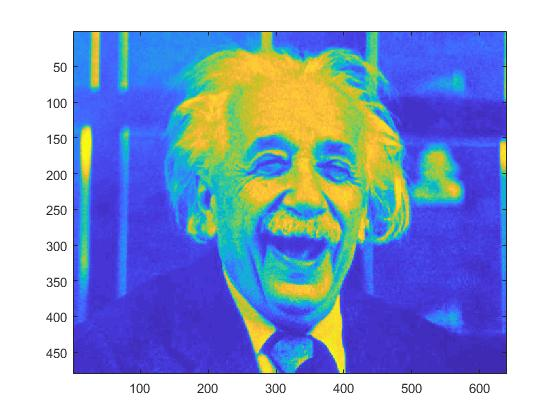
\includegraphics[scale=0.6]{reference_image.jpg}
    \caption{Reference image for comparison purposes}
    \label{fig:reference1}
\end{figure}

\begin{figure}[H]
    \centering
    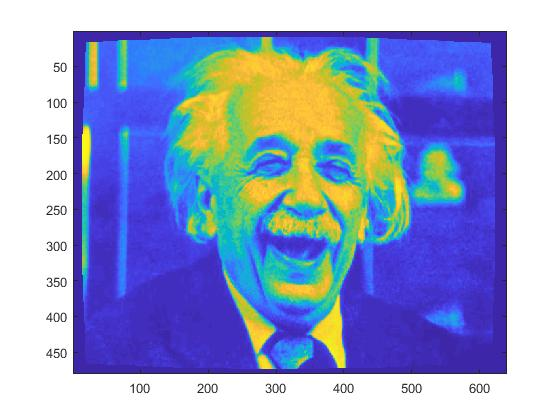
\includegraphics[scale=0.6]{partA.jpg}
    \caption{The distorted image "img01.tiff" which has been corrected for distortions}
    \label{fig:undist1}
\end{figure}

\section{Part B}
Part B deals with the correlation process only. The warp function parameters determined by the Matlab code are presented below.
\begin{align}
  u &= 5.03754\\
  \frac{\partial u}{\partial x} &= 0.04073 \\
  \frac{\partial u}{\partial y} &= -0.02176 \\
  v &= -1.03562 \\
  \frac{\partial v}{\partial x} &= -0.00915 \\
  \frac{\partial v}{\partial y} &= 0.03048
\end{align}
The corresponding correlation coefficients are
\begin{align}
  C_{ZNSSD} &= 0.005872084419686 \\
  C_{ZNCC} &= 0.997063957790157.
\end{align}
Both correlation coefficients have been presented here in order to illustrate that the $C_{ZNCC}$ coefficient is much easier to interpret. The determined warp function parameters were used to undeform the image "img02.tiff" to obtain figure \ref{fig:undist2}. Comparing this to the reference figure in figure \ref{fig:reference2} it can be seen that the determined warp function parameters are sufficiently accurate.

\begin{figure}[H]
    \centering
    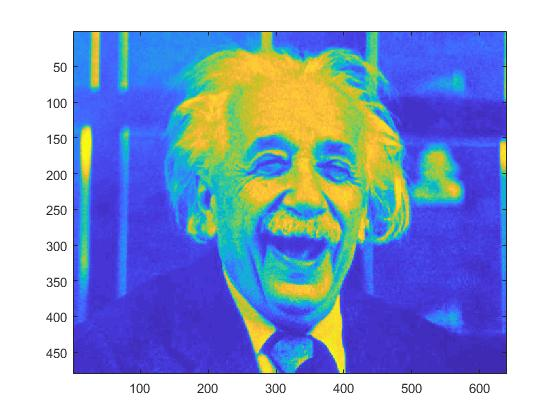
\includegraphics[scale=0.6]{reference_image2.jpg}
    \caption{Reference image for comparison purposes}
    \label{fig:reference2}
\end{figure}

\begin{figure}[H]
    \centering
    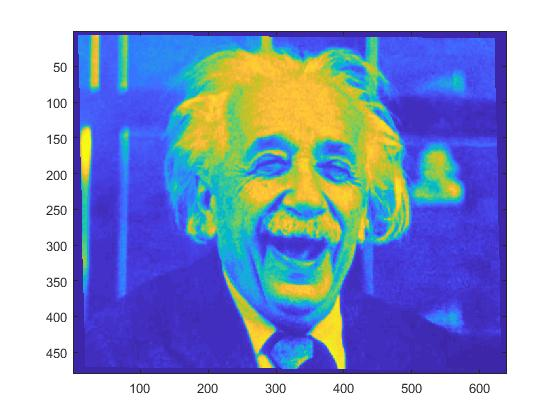
\includegraphics[scale=0.6]{partB.jpg}
    \caption{The distorted image "img01.tiff" which has been corrected for distortions}
    \label{fig:undist2}
\end{figure}
\section{Part C}
Part C combine both Part A and Part B. The calibration code of Part A is used to determine the calibration parameters for the camera system. These camera parameters are then used to undistort image "img03.tif" such that it is free of lens distortion. Then the correlation code is applied to this undistorted image in order to determine the warp function parameters. These warp function parameters are then used to undeform the image. This undeformed image is shown in figure \ref{fig:undist3}. Comparing this image to the original undistorted image in figure \ref{fig:reference3} it seems that a 

It is important to note that this method of using the calibration parameters to undistort the image prior to performing correlation on the image is not correct. This is because interpolation is used to undistort the image and additional interpolation is used within the correlation code. Thus by introducing an extra case of interpolation the reliability of the data is compromised.

\begin{figure}[H]
    \centering
    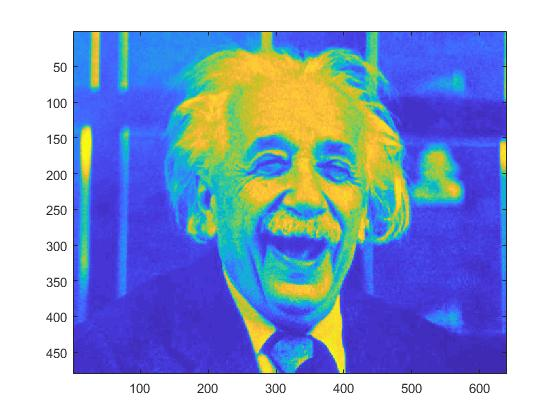
\includegraphics[scale=0.6]{reference_image2.jpg}
    \caption{Reference image for comparison purposes}
    \label{fig:reference3}
\end{figure}

\begin{figure}[H]
    \centering
    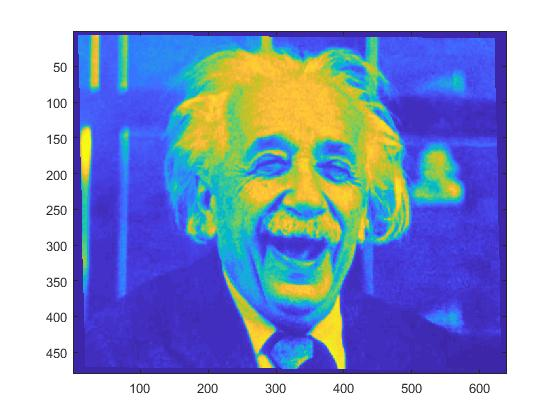
\includegraphics[scale=0.6]{partB.jpg}
    \caption{The distorted image "img01.tiff" which has been corrected for distortions}
    \label{fig:undist3}
\end{figure}

\chapter{Conclusion}
This document outlines the Digital Image Correlation process. It presents the background information on camera optics and the mathematical relation used to model these optics in a camera model. Thereafter the calibration process is discussed which determines the parameter values for the camera model. Correlation is then reviewed with focus on the inverse compositional Lucas-Kanade algorithm. Finally the results of the Matlab codes are given in order to illustrate that the methods presented here are correct.


\bibliography{references}
\bibliographystyle{plain}
\end{document}




% website for computer vision http://dblp.uni-trier.de/db/journals/ivc/ivc29.html


% Are you a vault dweller, cause you seem pretty S.P.E.C.I.A.L. to me





% https://drive.google.com/uc?export=download&confirm=TXgS&id=0B8ChoAcEOa4HbWxmbGFPV2M0aHM
% https://drive.google.com/uc?export=download&confirm=3xOY&id=0B8ChoAcEOa4HaEljZllabTZaeEk
% https://drive.google.com/uc?export=download&confirm=Lu4C&id=0B8ChoAcEOa4HcHZJMlZLeHdwdnc
% https://drive.google.com/uc?export=download&confirm=Qic1&id=0B2LiEl8up6X_R1V5NkF2NVhwaG8
% https://drive.google.com/uc?export=download&confirm=Qic1&id=0B2LiEl8up6X_R1V5NkF2NVhwaG8
% https://drive.google.com/uc?export=download&confirm=78XC&id=0B_q296AKMRsBUGtORW1jQ0lKQzQ


% https://drive.google.com/uc?export=download&confirm=cxmO&id=0B56v3YurenhzYTRXZGZ6MzJOWnc